\chapter{Systematic drug repositioning analysis}

\textbf{Key points}
\begin{itemize}
  \item The Functional Therapeutic Chemical Classification System (FTC) provides a descriptor for the function of drugs, which can be used to analyse the systematic relationship between function, structure and indication for approved drugs.
  \item Overall, approved drugs have dissimilar structures and dissimilar functions. When the therapeutic area is considered, the more specific the drug's indication is, the more similar the structure and function are. These observations are in line with the \emph{similar property principle} and can be used to isolate drug repositioning hypotheses from the dataset considered.
  \item A drug repositioning hypothesis is a pair of drugs indicated for different therapeutic areas (two ATC levels) but with a high functional similarity value. This method of extraction is called \emph{similarity-based}. I extracted 797 of such pairs and made them openly available through a web application.
  \item The set of repositioning hypotheses can be used to study the relationship between therapeutic areas: some repositioning hypotheses are more frequent between particular therapeutic groups and overlap with known off-label uses.
  \item From the full set of hypotheses, two use-cases are investigated in detail: hypertension and Alzheimer's disease. The drug \emph{similarity-based} repositioning hypotheses are compared against the \emph{toolbox approach}, where FTC categories are directly used as a starting point to forward repurposing opportunities.
  \item Cardiovascular hypertension hypotheses relate mostly to similar pharmacological actions but in different anatomical areas. Alzheimer's disease hypotheses involve biological processes related to the Tau protein and beta-amyloids; the majority of hypotheses find supporting evidence in the biomedical literature.
  \item This analysis concludes the thesis. Chapter 5 sets the work done in the context of the overall drug discovery process and discusses future work and open questions.
\end{itemize}

\textbf{Author's comment}

This chapter is a narrative analysis of the content of the FTC. Results and discussion are mixed together as I believe it makes the text more understandable and clarifies the reasoning behind the work. A methods section is provided at the end, describing the details of the analyses performed.

\hrulefill

\section{Introduction}
\label{sec:introduction}
I decided to look at drug repositioning from the perspective of the mode and mechanism of action (Chapter 1). The implementation of a solution required first some theoretical basis to be set, namely the black box model of the cell, specified using description logics (Chapter 2). The FTC then implemented the theory, as presented in the previous chapter (Chapter 3), and was evaluated against existing solutions to assess the relevance of the approach. This coming chapter will present the biological analysis performed over the content of FTC, in order to more directly address drug repositioning concerns.

As the FTC characterises the concept of function in a systematic fashion, the obvious questions to ask are: how does it relates to the chemical structure? Do similar compounds have similar functions? What about the indication? Is there any relation between function, structure and therapeutic usage?

In this regard, the analysis below first identifies the repositioning hypotheses present in the FTC and discusses the relevance of function in the process. Secondly, the extracted hypotheses are examined in depth and interpreted from a biological viewpoint. Because the FTC provides systemic insight on the drug repositioning topic, it is therefore possible to explore the broad relationship between therapeutic areas as well as the connection between drug repositioning and off-label uses. Finally, a couple of detailed use-cases are discussed: cardiovascular hypertension and Alzheimer's disease. These pathologies will serve to demonstrate how two different methodologies can be applied over the FTC to extract hypotheses: the \emph{similarity-based} and the \emph{toolbox} approaches.

This chapter is more focused on the biology and its interpretation. The content of FTC is dissected using semantic similarity and mode of action (MoA) cherry-picking. The conclusions drawn in this chapter will introduce future work to be done, as well as new leads to be explored.

\section{Structure, function and indication of drugs}
The most commonly accepted rule in drug discovery is probably the \emph{similar property principle}: similar structures have similar biological activities - or functions \citep{martin2002structurally} \citep{kubinyi1998similarity} \citep{johnson1990concepts}. Despite being true in some cases, there are plenty of examples in contradiction with this rule. As the FTC provides a unique characterisation of the function of chemical compounds, I decided to analyse the structure/function relationship for approved drugs, with a systematic stance. Before being able to do so, it is however necessary to choose adequate descriptors; the function will be represented by the FTC, but the structural descriptor still remains to be selected. This preliminary characterisation will allow me to then compare each drug's chemical structure against function in a systematic fashion and derive repositioning hypotheses.

\subsection{Structural descriptor selection}
\label{sec:structuraldescriptorselection}
The structure of two chemical compounds can be compared in a variety of ways, depending on the application \citep{johnson1990concepts}. In my case, the main motivation was to find a representative descriptor with a good dynamic range for the dataset considered - a thousand approved drugs. Moreover, the structural descriptor must be relatively easy to handle, fast to compute and with an explicit meaning, solely depending on the molecule and not on external factors.

In order to match these requirements, I decided to focus only on two-dimensional chemical structures, as numerous methods exist to compute them and because they are arguably more accurate for predicting target affinity than three-dimensional descriptors \citep{nettles2006bridging}, and therefore more suited to study bioactivity. The interpretation of the results is also easier and directly related to the chemical groups present in the structure \citep{todeschini2009molecular}.

Two-dimensional structures can be represented by fingerprinting methods (see section \ref{sec:structural}). Numerous implementations exist, varying in the chemical patterns encoded. I chose to try four of them over my dataset: hybridization, extended, MACCS and PubChem fingerprints (see section \ref{sec:structural}). These methods were selected because they are readily available in the Chemistry Development Kit \citep{steinbeck2003chemistry} and relatively different one from another, therefore providing independent yet comparable results. Figure \ref{fig4-1} illustrates this: the plot shows the density distribution of similarity values between pairs of drugs for the various fingerprinting methods considered (see section \ref{sec:structuralsimbet} and \ref{sec:agreement}).

\begin{figure}[H]
    \centering
    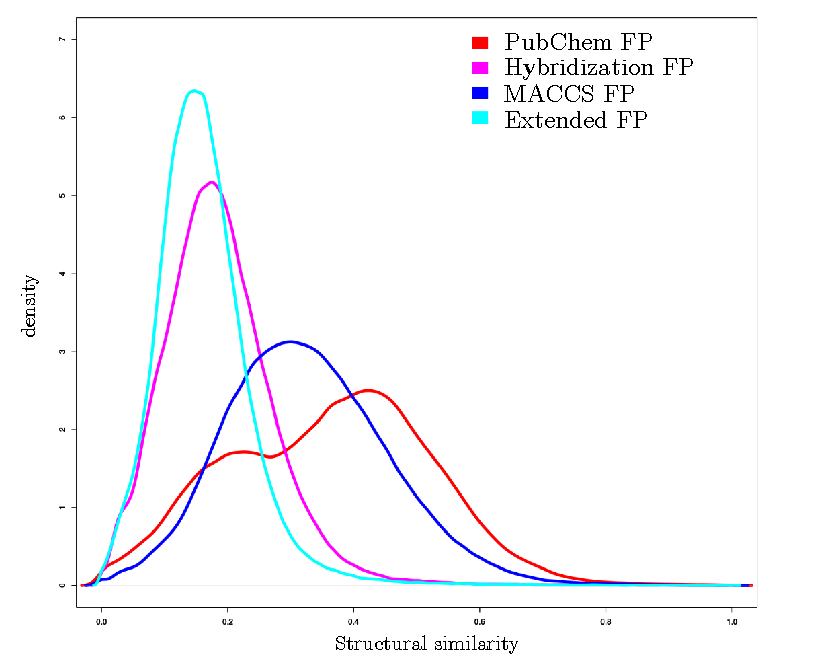
\includegraphics{fig4-1}
    \caption{Kernel density distribution for various chemical fingerprinting (FP) methods. All the methods have been applied as implemented in the CDK (cf section \ref{sec:agreement}). Each approved drug was compared against all other approved drugs (pairwise comparison), in order to determine which methodology provides the most suitable distribution to study the dataset.}
    \label{fig4-1}
\end{figure}

Different methods have different curves: MACCS and PubChem fingerprinting functions have wider distributions, as shown by the value of the interquartile range, higher than with the other methods (Table \ref{fpmethods}). The distribution of structural similarity values is an important criterion for this analysis, as it reflects the spread of the data. In my case, the wider, the more dynamic and therefore the better.

\begin{center}
\small
    \begin{tabular}{| l | l | l | l | l | l || l | l | l | l |}
    \hline
 & PubChem & Hybrid. & MACCS & Ext. & Mean corr. & Qu.1 & Mean & Qu.3 & Range \\ \hline \hline 
PubChem & X & 0.65 & 0.61 & 0.73 & 0.66 & 0.24 & 0.36 & 0.47 & 0.24 \\ \hline
Hybrid. & 0.65 & X & 0.66 & 0.84 & 0.72 & 0.13 & 0.19 & 0.24 & 0.11 \\ \hline
MACCS & 0.61 & 0.66 & X & 0.65 & 0.64 & 0.24 & 0.33 & 0.41 & 0.17 \\ \hline
Ext. & 0.73 & 0.84 & 0.65 & X & 0.74 & 0.11 & 0.16 & 0.2 & 0.09 \\ \hline
    \end{tabular} \captionof{table}{Pearson's Correlation values between various fingerprinting methodologies. ``Mean corr.'' stands for the mean value of the correlation coefficients. ``Ext.'' stand for Extended fingerprinter, ``Hybrid.'' for Hybridization. ``Range'' describes the interquartile range (Qu.3 - Qu.1), based on the similarity values.}
    \label{fpmethods}
\end{center}

Nonetheless, the agreement between the various fingerprinting methodologies also has to be considered: the goal is to find an average structural descriptor, somehow representative and not too polarised, in order to derive systematic conclusions later on. The agreement between methodologies was defined by the Pearson correlation coefficient (see section \ref{sec:agreement}) and is presented on Table \ref{fpmethods}. Briefly, this coefficient ranges between -1 to 1 and reflects how correlated two series of points are, 1 being a total positive correlation and -1 a total negative correlation. As each method is compared against all other fingerprinting methodologies, I considered the average of Pearson's coefficients as a representative metric; the higher the value, the more a method agrees with the others (``Mean corr.'' on Table \ref{fpmethods}). From this heuristic, table \ref{fpmethods} shows that the extended fingerprinting method is the most in line with the others (mean = 0.74), MACCS being the one agreeing the least (mean = 0.64). Nonetheless, all methods have pretty similar average values (see Table \ref{fpmethods}), meaning that all techniques reach overall the same level of agreement. Note that the extended and hybridisation fingerprints have the highest agreement value between them (0.84), reflecting the closeness in the implementation (personal discussion with CDK developers).

Based on these results, I decided to use the PubChem fingerprint to represent the chemical structure of drugs. The method distributes best the dataset analysed and agrees well with the other fingerprinting methodologies tested, features required for the subsequent drug repositioning analysis.

\subsection{Dissimilar structures have dissimilar functions}
The functional descriptor derives from the structure of the FTC and the semantic similarity. Given a pair of drugs, the closer they are present in the taxonomic tree, the more similar they are inferred to be (cf section 2.4.3). From this selection of the functional and structural descriptors, it is possible to study the relationship between drugs.

The similar property principle states that similar structures have similar biological activities. The rule was derived from QSAR analyses, where the goal is to try to fit a chemical structure inside a cavity, for instance the active site of an enzyme \citep{todeschini2009molecular}. In such a case, the rule is intuitively acceptable, yet numerous exceptions are known. The functional descriptor introduced can abstract away from this physical viewpoint and appreciate the similarity relationship in a systematic fashion. In this regard, Figure \ref{fig4-2} illustrates the distribution of similarity values for all pairs of drugs. Note that the indication is not taken into consideration at this stage.

\begin{figure}[H]
    \centering
    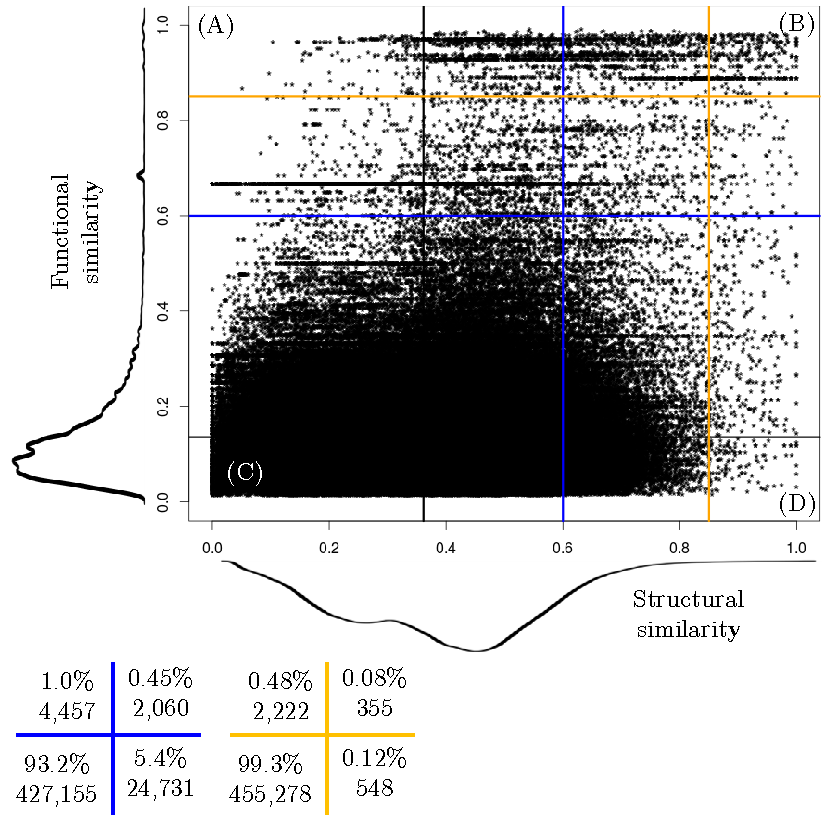
\includegraphics{fig4-2}
    \caption{Functional against structural similarity values for approved drugs. Each drug is compared against all other drugs (pairwise comparison) using both the structural and functional descriptors and corresponding to one dot or data point on the graph. Two different arbitrary thresholds are applied, represented by the blue and orange lines on the graph. The blue line separates the fairly similar values (\textgreater 0.6) from the rest, and the orange ones split up the highly similar (\textgreater 0.85) from the rest of the dataset. The graph is divided and labelled into 4 sections, identified by letters on the figure. The numbers of data points present in each one of these areas are listed on the table below the plot. The kernel density distribution are plotted on the side of the axis (qualitative) in order to appreciate the distribution of the data.}
    \label{fig4-2}
\end{figure}

The scatter plot is further divided into areas, broadly separating groups of drugs based on their relative similarity. I chose to consider two different thresholds, in order to separate the similar compounds from the dissimilar ones, represented by the blue and orange lines in Figure \ref{fig4-2}. The first threshold (blue) is set at an arbitrary similarity value of 0.6. This number appears able to separate the relatively similar from dissimilar compounds, and is derived from observations made in Figure 4-9. It also corresponds to the plateau values for both the structural and functional descriptors (Table \ref{fpmethods} and Table \ref{tablespecind}). The second threshold (orange line) was set at the arbitrary value of 0.85; it separates strongly similar compounds from the rest. This value is generally accepted as a cut-off (\cite{chemsimwiki} and personal discussions). The two thresholds reveal the same trend of data distribution (tables in Figure \ref{fig4-2}) in their different areas.

From the distribution of values on the graph, it is clear that the large majority of molecules have dissimilar structures and dissimilar functions. This corresponds to area C on the Figure \ref{fig4-2}, containing either 93\% or up to 99\% of the data points, depending on the threshold considered. This result can be explained as follows: approved drugs cover a wide range of different bioactivities (dissimilar functions), affecting numerous distinct processes involved in diseases. Their pharmacology is mediated via an interaction with different protein targets, therefore different chemical structures are needed. Moreover, for patent concerns, dissimilar structures are usually sought in order to maximise intellectual protection \citep{barratt2012drug}. This explanation is consistent with the low number of drugs with similar functions and similar structures (area B on the graph), pairs in agreement with the similar property principle.

Interestingly, a number of drugs are not in line with the similarity rule, represented by the data points in areas A and D. Such pairs have either similar functions with low structural resemblance (area A) or high structural similarities with little shared bioactivity (area D). This observation shows the challenge in drug discovery to relate function and structure: similar MoAs can be obtained with different structures (area A), and just because two structures are similar does not imply that they will trigger the same biological effect (area D).

Two conclusions can be derived from this plot. First, the graph reveals that most drugs have dissimilar structures and dissimilar functions, which I interpret as complementary and in line with the similar property principle. The relation between these pairs of compounds is not informative for drug repositioning and they can later be filtered out. Secondly, the plot enables the identification of exceptions to the similarity rule (areas A and D). These pairs of drugs are of particular interest, as they represent an unexpected pharmacology, not in line with the rule and therefore more difficult to identify. Such pairs are present in limited quantities, yet they intriguingly more numerous than the pairs respecting the principle and will be investigated in more detail.

Finally, on the Figure \ref{fig4-2}, it is possible to notice some artefactual horizontal straight lines, where the functional similarity is identical for a certain number of pairs (obvious one around functional similarity of 0.67 on Figure \ref{fig4-2}). Table \ref{table:lines} presents an illustration of the reason why such lines appear: when multiple drugs have the same set of FTC annotations, they end up having the same functional similarity value. For instance on Table \ref{table:lines}, the drugs guanfacine, lofexidine and dexmedetomidine all have the very same annotations. The drugs brimonidine, tizanidine and clonidine are also sharing the exact same set of FTC categories, therefore during the pairwise comparisons, the pairs will have the same functional similarity values. Note that the structural similarity still varies. In the example presented, the functional similarity values are relatively high (0.951219), reflecting the very tight similarity of actions between these compounds, acting on identical or very similar targets.

\begin{center}
\footnotesize
    \begin{tabular}{| p{2cm} | p{2cm} | p{4cm} | p{4cm} |}
    \hline
Structural similarity & Functional similarity & Drugs 1 (perturb Alpha-2A adrenergic receptor) & Drugs 2 (perturb Alpha-2A, 2B and 2C adrenergic receptor)\\ \hline \hline
0.331551 & 0.951219 & Guanfacine (DB01018) & Brimonidine (DB00484) \\ \hline
0.349515 & 0.951219 & Lofexidine (DB04948) & Brimonidine (DB00484) \\ \hline
0.42515 & 0.951219 & Guanfacine (DB01018) & Tizanidine (DB00697) \\ \hline
0.427807 & 0.951219 & Lofexidine (DB04948) & Tizanidine (DB00697) \\ \hline
0.5125 & 0.951219 & Dexmedetomidine (DB00633) & Clonidine (DB00575) \\ \hline
0.525974 & 0.951219 & Lofexidine (DB04948) & Clonidine (DB00575) \\ \hline
0.556818 & 0.951219 & Dexmedetomidine (DB00633) & Tizanidine (DB00697) \\ \hline
0.610169 & 0.951219 & Dexmedetomidine (DB00633) & Brimonidine (DB00484) \\ \hline
    \end{tabular} \captionof{table}{Extraction of data points of a horizontal lines present on Figure \ref{fig4-2}. The list of drugs 1 are all affecting the same molecular targets, and so are the drugs 2. As a result the functional similarity values are identical and constitute the lines observed. Note that structural similarity values ranges, reflecting the different chemical structure among these compounds.}
    \label{table:lines}
\end{center}

So far structure has only been compared to function; yet in order to be more meaningful, the indication of the drugs also has to be considered in the analysis. Intuitively, compounds present in the same therapeutic group should share higher similarity values, reflecting that they target related proteins and have more similar functions (section 3.5.2).

\subsection{The more specific an indication is, the more similar the function and structure are}
\label{sec:themore}
The ultimate value of a chemical compound arises from its therapeutic usage. In this regard, the legal indication of a drug is the gold-standard of information. This section further analyses the functional and structural descriptors introduced before and compares them against the legal indication and usage, as represented in the Anatomical Therapeutic Chemical Classification System (ATC). The goal of this comparison is to see whether the descriptors can further provide any meaningful information regarding the indication of a drug, which could be used to retrieve repositioning hypotheses.

According to the similar property principle, drugs present in the same therapeutic group should have on average relatively closer structures and functions. In order to validate this assumption, I considered the five hierarchical levels of the ATC as a representation of the specificity of the indication, with the first or top level of the ATC representing generic and broadly defined indications and the fourth level or bottom level characterising very precisely the indication of a compound (see Figure \ref{fig4-3}).

\begin{figure}[H]
    \centering
    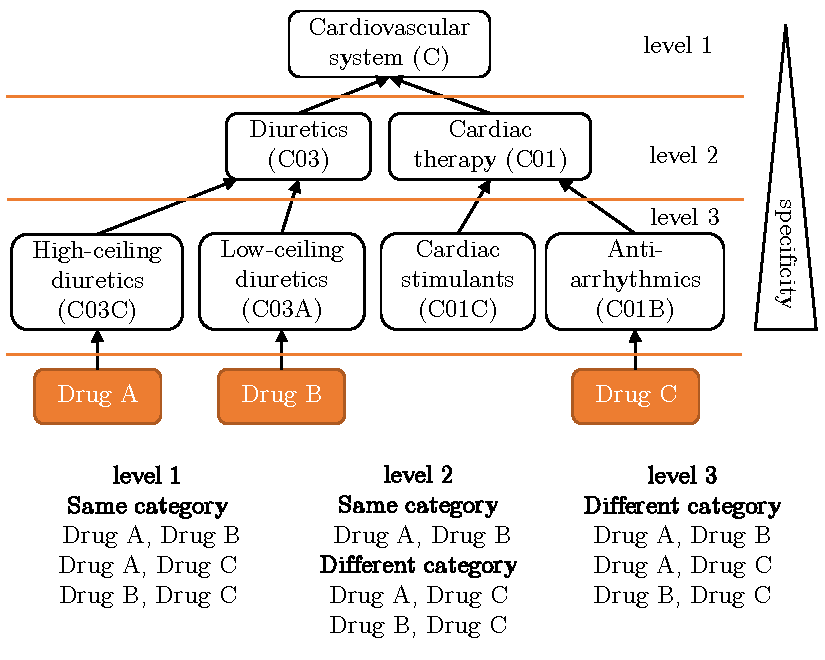
\includegraphics{fig4-3}
    \caption{Specificity of the indication of a drug as represented in the ATC. The ATC captures drug's indication and is organised over 5 levels (only 4 shown here for clarity), 1 being the highest and most generic level. When descending the tree, the specificity of the indication or action increases. Pairs of drugs can be flagged as belonging to either the same or different ATC category, depending on the level considered (resolution). Three examples are given on the figure in this regards, for the drugs A, B and C. For instance, when only the level 1 is considered, all pairs of drugs are present in the same category (\emph{Cardiovascular system}). When the level 2 is considered, the pair of drugs A and B still belong to the same category (\emph{Diuretics}), but these two drugs are not sharing the indication of drug C, \emph{Cardiac therapy}. At a resolution of the level 3, each drug has a separate indication/action.}
    \label{fig4-3}
\end{figure}

It is possible to use this definition of the specificity of an indication to filter pairs of drugs and look at the overall evolution of structural and functional similarities. Such an analysis is shown in Figure 4-4, where only pairs of drugs sharing a common indication are shown. When the specificity of the indication increases, represented by the increasing number of the ATC level considered, the average functional and structural similarity increases too.

\begin{figure}[H]
    \centering
    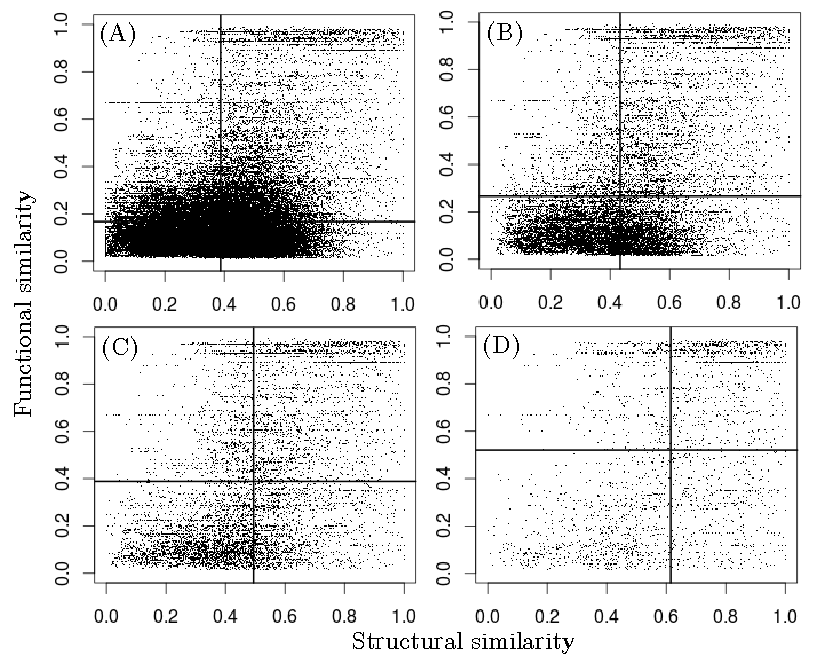
\includegraphics{fig4-4}
    \caption{Distribution of the functional and structural similarity values for pairs of drugs present in the same ATC categories (same indication). The different panels reflect the increasing specificity of the indication of the drugs. X axes is the structural similarity and Y axes is the functional similarity (calculated as with previous graphs). (A) 1 ATC level resolution. (B) 2 ATC level resolution. (C) 3 ATC level resolution. (D) 4 ATC level resolution. Conceptual explanation of resolution and levels is available on Figure \ref{fig4-3}. When the specificity of the indication increases (resolution increasing), the average functional and structural similarity values increases too (black lines).}
    \label{fig4-4}
\end{figure}

On the contrary, when only pairs of drugs indicated for increasingly different indications are compared, the average similarity stays the same, as shown on Figure \ref{fig4-5} and summarised Table \ref{tablespecind}.

\begin{figure}[ht]
    \centering
    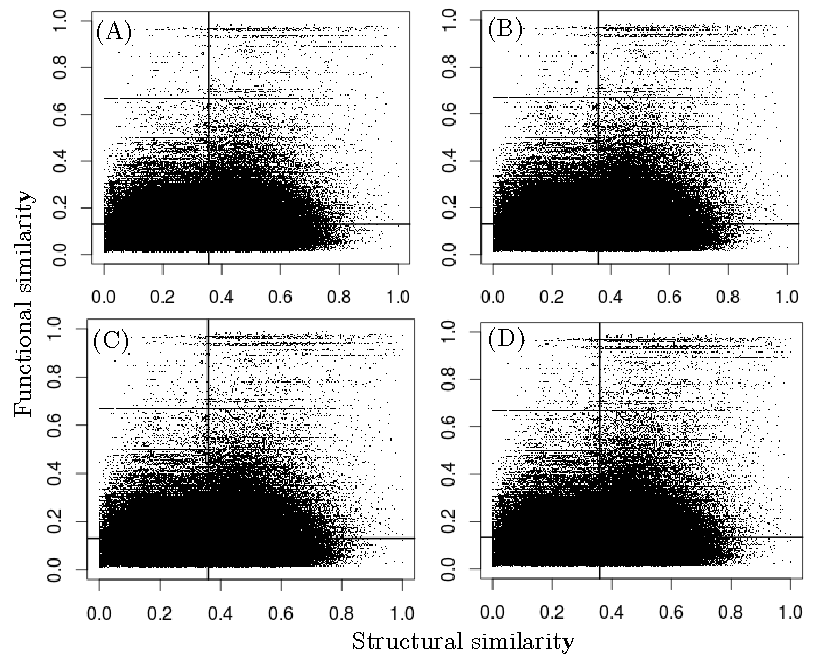
\includegraphics{fig4-5}
    \caption{Distribution of the functional and structural similarity values for pairs of drugs present in different ATC categories (different indication). The different panels reflect the increasing specificity of the indication of the drugs. X axes is the structural similarity and Y axes is the functional similarity (calculated as with previous graphs). (A) 1 ATC level resolution. (B) 2 ATC level resolution. (C) 3 ATC level resolution. (D) 4 ATC level resolution. Conceptual explanation of resolution and levels is available on Figure 4-3. When the specificity of the indication increases (resolution increasing), the average functional and structural similarity values stays identical (black lines).}
    \label{fig4-5}
\end{figure}

Figures 4-6 and 4-7 respectively show the kernel densities of the structural and functional similarities values for the pairs of drugs sharing an indication at a given ATC level. Note that the two descriptors have different behaviours. The structural similarity appears centred in the middle of the graph, and slowly evolves towards higher similarity values with indication specificity. A jump is observed from level 3 to 4 (brown curve on Figure \ref{fig4-6}), and is manifested by a larger increase in the average value. This observation is explained by the very definition of the indication coming from the ATC: level 4 handles the categorisation of drugs based on their chemical structures (cf section 3.2.6), therefore it is more likely for a pair of molecules present in the same fourth level ATC category to have very similar structures.

\begin{center}
\small
    \begin{tabular}{| l | l | l | l | l | l |}
    \hline
 & Specificity of indication (ATC level): & 1 & 2 & 3 & 4 \\ \hline \hline
Same indication & Average structure similarity & 0.39 & 0.43 & 0.49 & 0.62 \\ 
 & Average function similarity & 0.17 & 0.27 & 0.39 & 0.52 \\ \hline
Different indication & Average structure similarity & 0.36 & 0.36 & 0.36 & 0.36 \\
 & Average function similarity & 0.13 & 0.13 & 0.13 & 0.13 \\ \hline
    \end{tabular} \captionof{table}{Evolution of the specificity of indication with the ATC levels. Increasingly similar indications have increasingly similar functional and structural values. The functional and structural similarity values are not evolving when increasingly different indications are considered.}
    \label{tablespecind}
\end{center}

\begin{figure}[H]
    \centering
    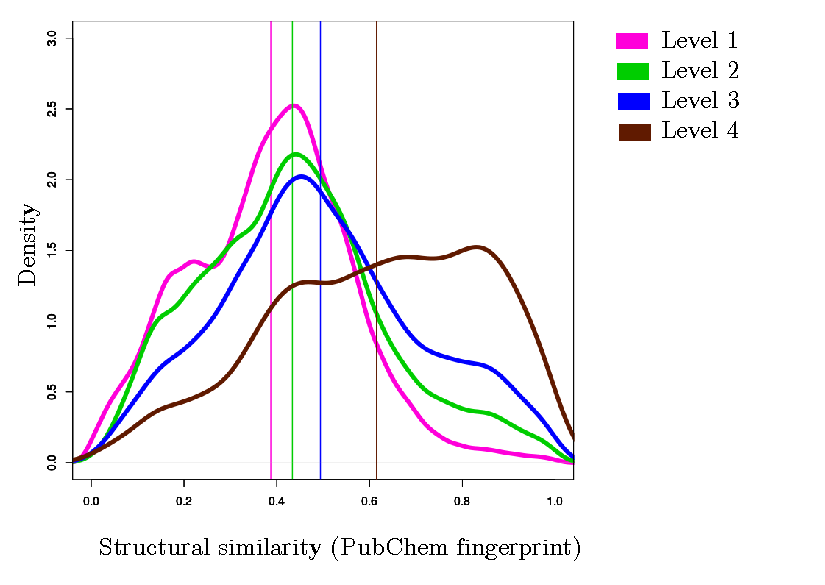
\includegraphics{fig4-6}
    \caption{Kernel density distribution of the structural similarity values for drugs sharing an indication. All ATC categories have been considered. Each curve represent an ATC resolution level, as indicated on the legend. Conceptual explanation of resolution levels is available on Figure \ref{fig4-3}. Solid vertical lines are the corresponding means. This graph shows that with an increasingly specific indication (increasing resolution) the average structural similarity values increase too.}
    \label{fig4-6}
\end{figure}

The functional similarities steadily increase on average (see Table \ref{tablespecind}). With this descriptor, the relative changes in similarities between different ATC levels are more located on the extremes, as shown in figure \ref{fig4-7}: when the specificity of the indication increases, the number of low similarity values decreases, giving relatively more weight to the high ones.

\begin{figure}[H]
    \centering
    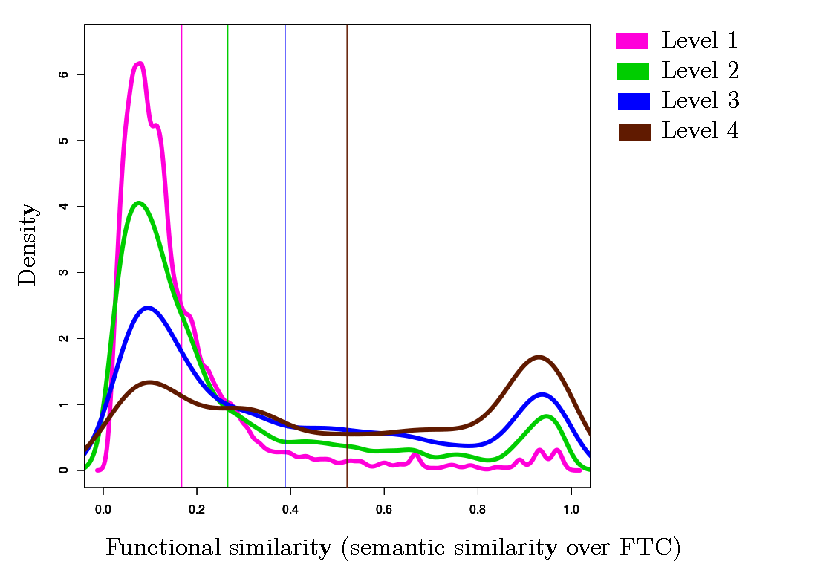
\includegraphics{fig4-7}
    \caption{Kernel density distribution of the functional similarity values for drugs sharing an indication. All ATC categories have been considered. Each curve represent an ATC resolution level, as indicated on the legend. Conceptual explanation of resolution levels is available on Figure \ref{fig4-3}. Solid vertical lines are the corresponding means. This graph shows that with an increasingly specific indication (increasing resolution) the average functional similarity values increase too. See Table \ref{tablespecind} for values.}
    \label{fig4-7}
\end{figure}

Taken together, these results confirm the similarity principle at a systematic scale: on average, drugs with closely related indications are structurally and functionally similar, as captured by the descriptors used. As an example, the plot showed in Figure \ref{fig4-4} panel D displays the highest average similarity, when the indication is the most specific (highest ATC level). This average similarity value was used to set the threshold level at 0.6 in Figure \ref{fig4-2}; it separates functionally similar compounds from the rest.

Still on the panel \ref{fig4-4}-D, it is possible to observe the limit of the structural similarity to predict pharmacologically related molecules. The pairs of this area have indeed closely related indications and high functional similarity as expected, yet a very low structural resemblance. The Figure \ref{fig4-8bis} shows a representative pair in details: isothipendyl (DB08802) and bromodiphenhydramine (DB01237) are both anti-histamine compounds and share a high functional similarity (0.93), yet they have different chemical scaffold, resulting in a very low structural similarity (0.30). The biological relatedness of such molecules would be missed by considering their molecular features alone, yet the FTC enables it.

\begin{figure}[H]
    \centering
    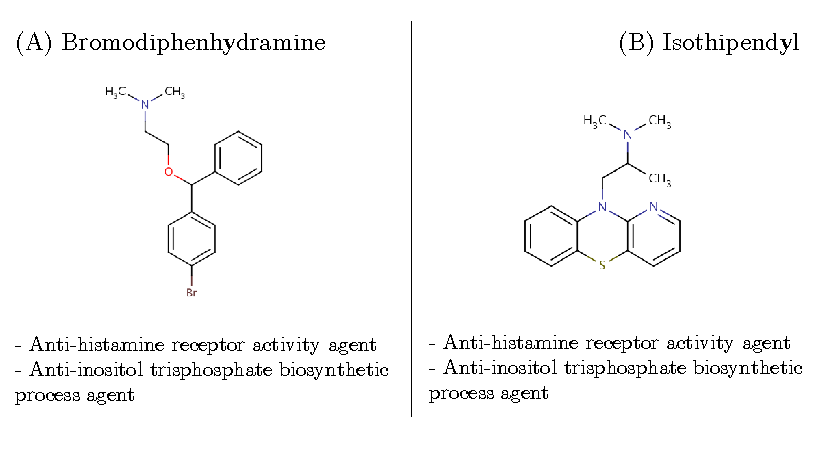
\includegraphics{fig4-8bis}
    \caption{Example of pair of drugs with low structural and high functional similarity values, classified in the same ATC category and used for the same clinical indication (\emph{Antihistamines}). (A) Chemical structure and list of FTC categories inside which the isothipendyl was classified. (B) Molecular structure and list of FTC categories inside which the bromodiphenhydramine molecule was classified. These two drugs share all FTC categories (functional similarity = 0.93), yet their molecular structures are dissimilar (structural similarity = 0.30).}
    \label{fig4-8bis}
\end{figure}

Interestingly, still on the Figure \ref{fig4-4}-D, some of the pairs still have low similarity values (structural and functional lower than 0.3); these points are outliers to the similar property principle and reflect the limits of the descriptors. I performed an error analysis in order to identify the reasons behind the non-respect of the rule by these drugs. The pair of drugs dipyridamole and epoprostenol is a good illustration of the most common cases of misclassification. These two drugs have a relative functional similarity of 0.10 and a structural similarity of 0.14, despite being both categorised as \emph{Platelet aggregation inhibitors} in the ATC (code: B01AC). Although resulting in the same biological outcome and clinical usage, these two drugs are mainly targeting different proteins, a phosphodiesterase in the case of dipyridamole and the P2Y purinoceptor 12 in the case of epoprostenol. In order to interact with these receptors, two different chemical structures are needed and it is therefore expected that the two molecules would have different structures (see Figure \ref{fig4-8}). However, the MoAs from the FTC are not shared either, which comes from missing annotations on the protein targets or because the molecular root of the effect is unknown. It is therefore also not possible to relate these two drugs based on their functions, because of lack of recorded knowledge.

\begin{figure}[H]
    \centering
    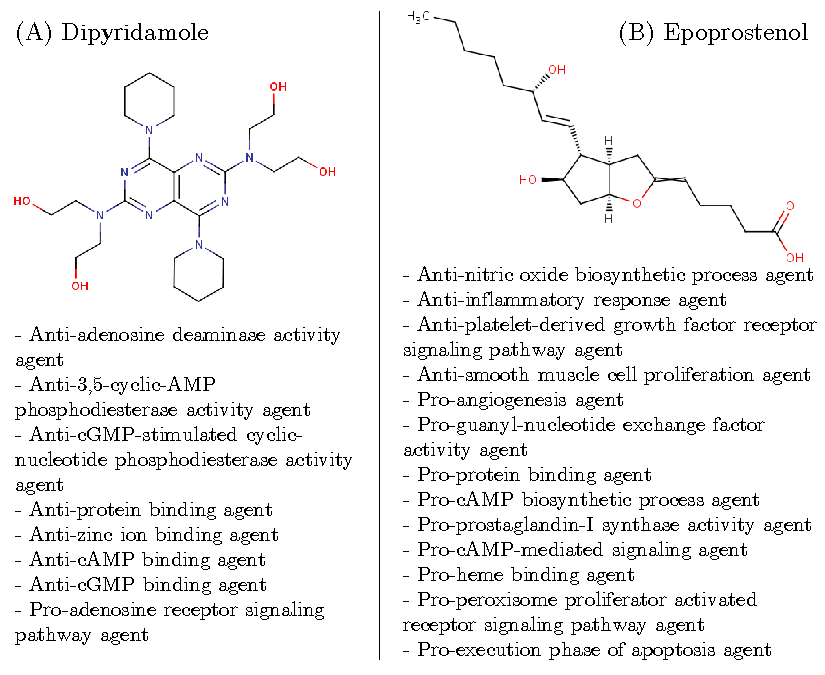
\includegraphics{fig4-8}
    \caption{Example of pair of drugs with low structural and functional similarity values, yet classified in the same ATC category and used for the same clinical indication (\emph{platelet aggregation inhibitors}). (A) Chemical structure and list of FTC categories inside which the dipyridamole was classified. (B) Molecular structure and list of FTC categories inside which the epoprostenol molecule was classified. These two drugs do not share any of the FTC categories listed (functional similarity = 0.10) and their molecular structures are dissimilar (structural similarity = 0.14).}
    \label{fig4-8}
\end{figure}

The figures presented in this section show an observation of primary importance for drug repositioning: the computational descriptors used are able to serve as a proxy for the expected behaviour of the concepts of function and structure in regards to the real clinical indication of a drug. The more similar a pair of drugs are based on either their functional or structural features, the more likely these drugs are clinically indicated for the same sets of diseases.

Note that the data analysis shown in the two previous sections only identified average patterns; particular data points were not taken into considerations. Some exceptions or outliers exists, which will be considered as starting points to formulate drug repositioning hypotheses.

\subsection{Isolation of drug repositioning hypotheses}
\label{sec:isolation}
As motivated before (section 3.2.6), the ATC can be considered as a gold standard resource for representing the therapeutic area of a drug. The second level of this classification system in particular represents the clinical indication of a compound well \citep{world2006anatomical}; it is not too specific to capture the MoA and exact pharmacology, yet still biologically meaningful and not too abstract. Example of second level ATC categories are: \emph{Anabolic agents for systemic use} (A14) and \emph{Anti-haemorrhagics} (B02). I and others (\cite{campillos2008drug}, \cite{napolitano2013drug}) have considered that drugs categorised under different second-level ATC codes can be considered as indicated for different diseases.

Drugs used in the treatment of different conditions are expected to have dissimilar functions, as in principle such agents affect separate biological processes, themselves related to distinct diseases. The graph in Figure \ref{fig4-9}-A recounts this statement: as expected most of the pairs have low structural and functional similarity values.

\begin{figure}[ht]
    \centering
    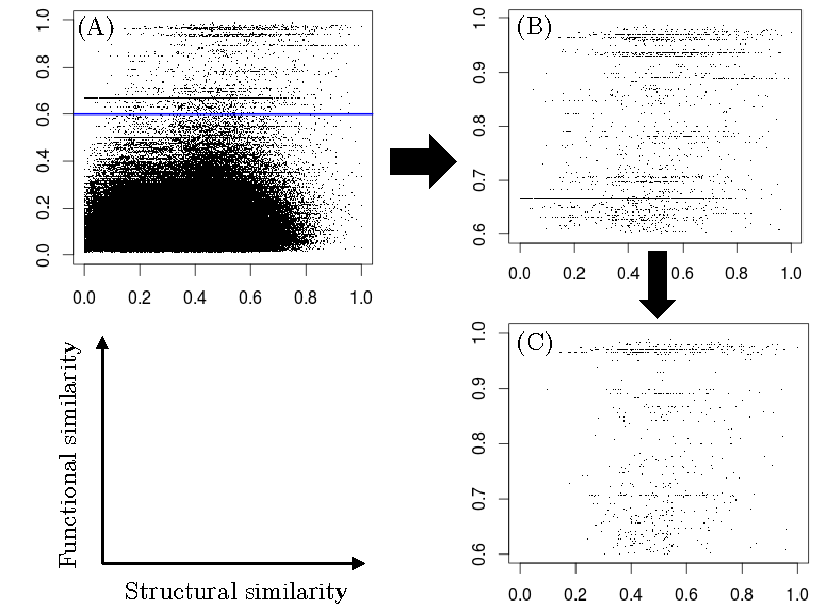
\includegraphics{fig4-9}
    \caption{Isolation of drug repositioning hypotheses. (A) All the pairs of drugs classified in different ATC categories (level 2 resolution) are plotted (identical plot as Figure 4-5 panel B). The blue line is the threshold above which pairs are functionally similar but are indicated for different usage according to the ATC. (B) Zoom on the data set above the blue line. (C) Pairs of drugs with little recorded knowledge are discarded from the analysis (see material and method). This set of data represents the repositioning hypotheses and are featured in the web application.}
    \label{fig4-9}
\end{figure}

However, some data points on this plot have relatively high functional similarity values (similarity superior to 0.6, identified by the blue line). These pairs of drugs are unexpected; such compounds appear to be strongly related on the functional level, yet in practice they are clinically used for radically different indications. Such data points have been interpreted as repositioning hypotheses.

In this regard, the values shown above the blue line (0.6) in Figure \ref{fig4-9}-A have been first isolated (see Figure \ref{fig4-9}-B). Some drugs with little knowledge have been discarded (low number of annotations - see section \ref{sec:filteringof}); the remaining set is displayed in panel (C). The pairs of molecules in the area Figure \ref{fig4-9}-C, defined as drug repositioning hypotheses, were isolated from the rest of the data points and further displayed through a web application (\url{https://www.ebi.ac.uk/chembl/research/ftc-hypotheses/}) in order to facilitate their exploration and validation.

A total of 797 pairs of points or repositioning hypotheses were considered. The hypotheses are grouped by therapeutic areas in the web application. For example, the ATC category J01 - \emph{Antibacterials for systemic use} contains 72 associations or potential drugs that are not indexed as antibacterial and yet could be used as such, based on their known role in the human body (\url{https://www.ebi.ac.uk/chembl/research/ftc-hypotheses/code/J01}). The web application further provides an aggregation of the ATC categories related to the one currently investigated. For instance the hypotheses related to the category \emph{Antibacterials for systemic use} are from drugs present in the ATC group L01 - \emph{Antineoplastic agents} (54 hypotheses), S02 (\emph{otologicals}, 16 hypotheses), V03 (\emph{All other therapeutic products}, 9 associations), D06 (\emph{Antibiotics and chemotherapeutics for dermatological use}, 9 hypotheses) and S03 (\emph{Ophthalmological and otological preparations}, 8 hypotheses).

Very often, the same drug is involved in multiple hypotheses. For instance, the antibiotic pefloxacin is functionally similar to 9 other drugs; this results in a network of interconnected drugs related to one therapeutic category. From the web application, it is possible to export the file containing hypotheses to further analyse the graph in Cytoscape \citep{shannon2003cytoscape}, a program commonly used to visualise networks and systems. These graphs will be extensively discussed in the rest of this chapter.

From the relationship between the structure, function and indication of approved drugs, it is possible to isolate outliers not following the predicted behaviour. Such data points extracted from the analysis have been defined as drug repositioning opportunities and are available via a web interface. Next sections will focus on particular therapeutic groups and use-cases, in order to identify the relevance and the limits of the approach.

\section{Open drug repositioning hypotheses}
\label{sec:opendrug}
The ATC provides data regarding the anatomical group inside which a drug has been assigned (first level) as well as its main therapeutic area (level 2). I considered this information as a gold standard defining the indication of a drug. As a reflection of polypharmacology, some of the drugs are already present in multiple ATC categories, or have multiple indications. For instance, acetylsalicylic acid is classified as a stomatological preparation (A01), an antithrombotic agent (B01) and an analgesic (N02), according to the various roles it can play in the human body. The hypotheses generated render a similar result: drugs are predicted to be active in other ATC categories on top of the ones they have already been manually assigned to.

The aim of this section is to characterise and interpret the hypotheses; indeed, before moving forward to perform laboratory experiments, it is necessary to have a clearer idea of the molecular reasons behind the predictions.

First I will present an overview of the hypotheses and illustrate how drug repositioning relates to the non-regulated uses of drugs. This topic is known as off-label uses \citep{offlabelwiki} and concerns around 20\% of the drug's prescriptions \citep{stafford2008regulating}. An off-label use is the indication of a drug for a non-regulated usage, either in terms of therapeutic group, dosage or patient group. This practice is legal in most countries, yet as it is non-regulated there is little information about it.

Secondly, I will investigate drug repositioning hypotheses for cardiovascular hypertension and Alzheimer's disease. These use-cases are also an opportunity to compare the hypotheses generated using functional similarity (section \ref{sec:isolation}) against the \emph{toolbox} approach, which considers drugs classified inside FTC categories directly as relevant for a biological process.

\subsection{Relationship between therapeutic areas}
In the context of this work, a repositioning hypothesis is defined as \emph{a pair of drugs that are functionally similar yet currently indicated for different clinical purposes}. In practice, this relationship can serve to relate therapeutic groups: some hypotheses are present more often than others between two given groups, providing insights as to how close these clinical areas are. In this respect, Figure 4-10 shows the association between therapeutic areas, with a resolution of two ATC levels.

\begin{figure}[H]
    \centering
    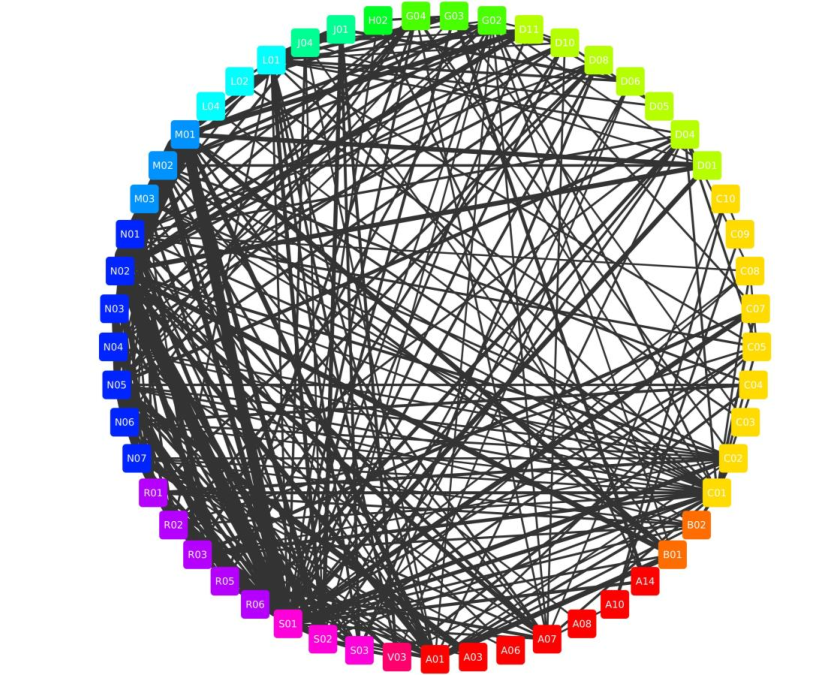
\includegraphics{fig4-10}
    \caption{Raw associations between therapeutic areas. All the repositioning hypotheses between two a therapeutic groups are merged to define the strength of association amongst these groups. The boldness of the line is directly proportional to the strength of association. For instance, there exists more repositioning hypotheses between the groups M01 and S01 (very bold line) than between the groups C10 and A07 (thinner line). Categories are sorted on alphabetical order and the colour is assigned based on the first letter of the group (therapeutic area). All the group S is pink for instance (S01, S02 and S03).}
    \label{fig4-10}
\end{figure}

It is rather challenging to derive any meaningful conclusion from the graph, yet the hairball reveals an interesting features of the dataset: a high inter-group connectivity, which appears stronger in some cases and weaker in others. For instance, D categories (dermatologicals) are less well connected than N series (nervous system), simply from visual observation. In order to simplify the problem faced and extract the essence of the dataset, I further decided to group categories considering solely their first ATC level and filtering out weak associations (cf methods section \ref{sec:filteringofthe}). The result is shown in Figure \ref{fig4-11}.

\begin{figure}[H]
    \centering
    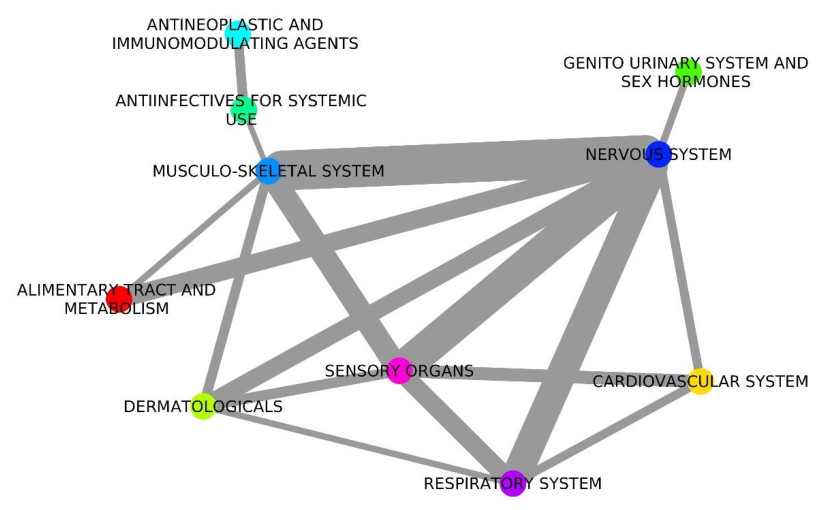
\includegraphics{fig4-11}
    \caption{Filtered and abstracted associations between therapeutic areas. The network is built from the data point shown on Figure 4-10. ATC categories have been grouped based on their first level: for instance all the hypotheses for the groups S01, S02 and S03 have been merged as S (or \emph{sensory organ} in this figure). Moreover, only the links involving a minimum of 25 hypotheses (arbitrary) have been kept in order to filter out the weak associations. The network shows the areas subject to drug repositioning or for which there exists a ``promiscuous'' pharmacology, which can be captured by the degree of a node (number of connections with other nodes).}
    \label{fig4-11}
\end{figure}

The resulting graph abstracts away details and shows clearer high level associations between groups. The most connected node is the nervous system (degree of 6). The high connectivity around this therapeutic area could be interpreted as the presence of numerous repositioning hypotheses; however, it is much more likely to be due to off-label usages. Neurology is a domain particularly famous for this \citep{cras2007off}. For instance, it is genuinely difficult to define and quantify concepts such as \emph{pain} \citep{bonica1979need} or any mental illness, therefore clinicians do not always use the officially indicated drug, depending on their diagnostic, personal experience and history of the patients (personal discussion with clinical pharmacologists).

Other therapeutic areas such as the ones related to sensory organs, dermatology and the musculoskeletal system are also well connected (degree of 4 and 5). The presence of the musculoskeletal category can be explained by the promiscuity of anti-inflammatory agents; usually such drugs are also active on the nervous system, explaining the strong relation between these two groups. This high level overview can be refined with the help of Figure \ref{fig4-12}.

\begin{figure}[H]
    \centering
    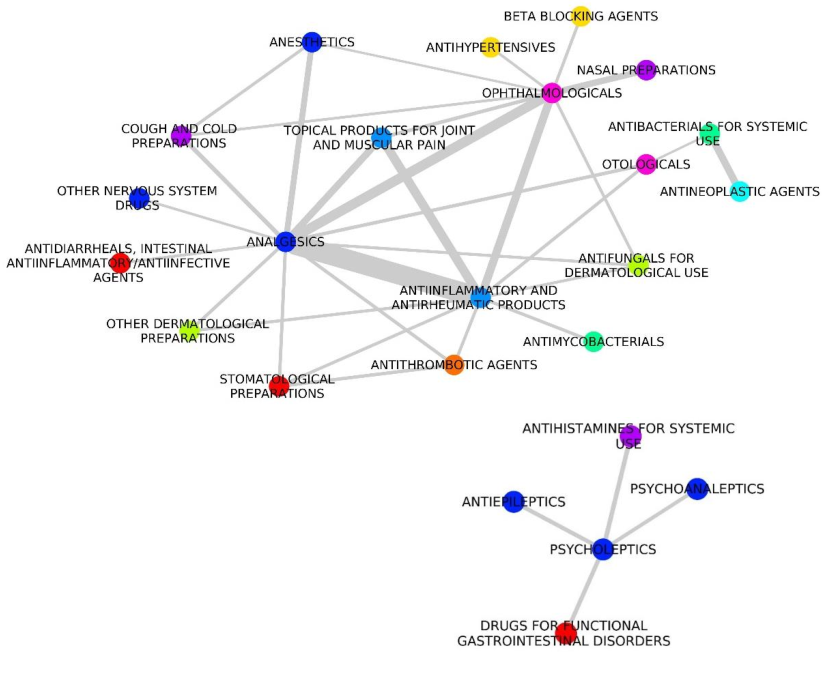
\includegraphics{fig4-12}
    \caption{Filtered associations between therapeutic areas. The network is built from the data point shown on Figure \ref{fig4-10}. Weak associations (less than 15 hypotheses) have been filtered out. The graph shows the high level association between therapeutic areas, for a two ATC level resolution. See text for interpretation of the edges.}
    \label{fig4-12}
\end{figure}

These graphs focus on the ATC level 2 indications, as in Figure \ref{fig4-10}, but with weaker associations filtered out (section \ref{sec:filteringofthe}). This more granular view of the data confirms the fussiness around neurological compounds; 6 out of 26 categories are from this therapeutic area and are well connected to the other nodes. Some associations are of special interest, as summarised in Table \ref{higlevelhypo} .

\begin{table}[htbp]
\scriptsize
\begin{tabular}{|l|l|p{5cm}|}
\hline
\multicolumn{2}{|c|}{\textbf{Therapeutic groups association}} & \multicolumn{1}{c|}{\textbf{Interpretation}} \\ \hline
Cough and cold & Analgesics & Analgesics are used in cough preparations \citep{atcr05} \\ \hline
Anti-inflammatory & Antimycobacterials & No naive interpretation \\ \hline
Analgesics & Ophtalmological & \multicolumn{ 1}{l|}{Related MoA, regulation of blood pressure} \\ \cline{ 1- 2}
Ophtalmological & Nasal preparation & \multicolumn{ 1}{l|}{} \\ \cline{ 1- 2}
Antihypertensive & Ophtalmological & \multicolumn{ 1}{l|}{} \\ \cline{ 1- 2}
Beta blocking agent & Ophtalmological & \multicolumn{ 1}{l|}{} \\ \hline
Antibacterial & Antineoplastic & Ortholog targets, replication of DNA \\ \hline
Antihistamines & Psycholeptics & Drowsiness, specially with first and second generation \citep{gengo1987antihistamines} \\ \hline
Gastrointestinal disorder & Psycholeptics & Currently used as treatment, preparations contain psycholeptics \citep{atca03} \\ \hline
Analgesics & Anti-inflammatory & Side-effect, shared bioactivity \citep{hunskaar1987formalin} \\ \hline
\end{tabular}
\caption{High level association between therapeutic groups and shared pharmacology. See Figure \ref{fig4-10} for source network.}
\label{higlevelhypo}
\end{table}

Analgesics (relief from pain) are strongly associated with cough and cold preparations. This pair is not so surprising; anti-flu medicines often mediate their effect as palliative pain killers, as confirmed in the ATC description of the category \citep{atcr05}. The strong connection between anti-inflammatory drugs and analgesics observed in the Figure 4-10 is confirmed; compounds from either of these classes are known to have overlapping pharmacology \citep{hunskaar1987formalin}. This relationship is further supported by the extra links to \emph{topical products for joint and muscular pain}, showing the ambiguity of biological action and the relatedness of these indications.

Another neurological category, psycholeptics (calming effect), is related to antihistamines and drugs for gastrointestinal diseases. The former association explains the drowsiness side-effect provoked by first and second antihistaminic agents. For gastrointestinal disorders, the link is explainable by the fact that psycholeptics are often administered as a palliative solution for such dysfunctions \citep{atca03}. An edge also connects stomatological preparations to analgesics, supporting this observation.

The strong relation between anti-neoplastic agents and anti-bacterials can be explained by the orthology between the proteins targeted by these drugs, namely the DNA replication machinery. The replication apparatus of bacteria and humans are still fairly similar \citep{hurle2013computational}, therefore a drug inhibiting one can also inhibit the other.

Ophthalmologicals are connected to cardiovascular drugs (beta blocking and antihypertensives agents) as well as to nasal preparations. This hub originates because of the shared fundamental MoA between all these categories: regulation of blood pressure and flow, in different systems. The functional similarity between these categories is high, as the pharmacological effect is mediated via the same biological process, yet the administration and delivery of the drug in the body leads to the specificity of the indication. This relationship will be analysed in more details in coming sections.

Finally, some of the edges are difficult to interpret without looking at the underlying pairs of drugs. For instance, the association between anti-inflammatory and anti-mycobacterial agents is unusual and requires deeper investigation to be interpreted (not discussed in this document).

This overview of the relationship between therapeutic groups reveals some expected associations, confirming the validity of the approach. Some known cases are represented in the graphs shown and are documented in the scientific literature. Polypharmacology between groups appears non-homogeneous, as some therapeutic areas are closer than others in terms of functional similarity and strength of association. The list of drug repositioning hypotheses contains some off-label pairs, which are drugs known and already used for an alternative indication yet not formally approved for it.

From this generic presentation of the dataset and in order to better characterise the repositioning hypotheses, I decided to focus in more detail on agents active for treatment or prevention of cardiovascular hypertension. Finally I demonstrate how the categories of the FTC can be used as a starting point to address Alzheimer's disease (toolbox approach).

\subsection{Drug repositioning for hypertension and the cardiovascular system}
The beginning of this chapter (section \ref{sec:themore}) compared pairs of drugs considering the relative similarity of their functions and structures. The closeness between two roles was defined as the semantic similarity over the content of the FTC; such a metric helped to identify related compounds, forward repositioning hypotheses and look at the relationships between therapeutic groups. This approach, referred to as \emph{similarity-based}, is useful when a known therapeutic category already exists in the gold standard (ATC) which can be used as a starting point for further investigations.

Complemenlarly, the FTC can also be directly used as a toolbox, in order to find drugs to fix or repair a molecular machinery; some FTC categories contain active molecules in theory capable of producing the described pharmacological effect. Therefore, knowing the desired MoA can help to identify what molecule to use for a particular condition. This methodology is named the \emph{toolbox approach}. The difference between the two approaches are illustrated and summarised in Figure \ref{fig4-13}.

\begin{figure}[ht]
    \centering
    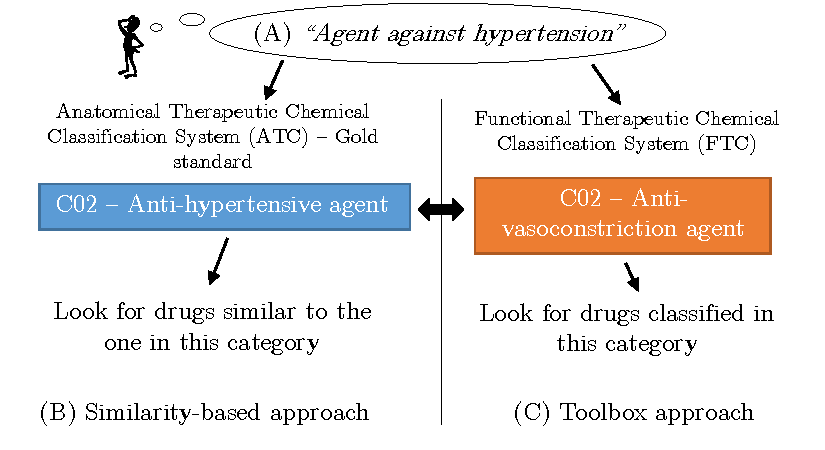
\includegraphics{fig4-13}
    \caption{Comparison of the similarity-based against toolbox approach for drug repositioning hypotheses investigation. (A) The concept formulated in natural language as in the head of a researcher or mentioned in a text is formalised and mapped to a term from a classification, either the ATC or the FTC in this case. (B) Similarity-based approach: the drugs functionally similar (semantic similarity over the FTC) to the ones listed in the ATC category are the drug repositioning hypotheses (displayed in the web application). (C) Toolbox approach: the drugs classified under the selected FTC category are capable of producing the MoA of interest. These compounds have been automatically assigned to the categories during the reasoning step (see Chapter 3 section 3.2.5). Note that often the ATC and FTC category have equivalent meanings, as emphasized by the bold black arrow between the categories.}
    \label{fig4-13}
\end{figure}

This section demonstrates how the FTC and the previously generated drug repositioning hypotheses can be used in practice, using hypertension as an example.

High blood pressure, or hypertension, is a medical condition leading to an increased risk of strokes, heart attacks and cardiovascular diseases \citep{law2003lowering}. In Europe alone, this condition is considered epidemic; hypertension affects between 30 to 45\% of the whole population \citep{swedberg2005task}, making it one of the leading causes of death. From a mechanistic perspective, hypertension can be straightforwardly regulated by lowering the blood pressure in the affected patient; this biological outcome can however be achieved in a variety of ways. For instance, the physical contraction of cardiac cells can be directly inhibited by blocking a receptor, the signalling pathway triggering the vasoconstriction can be perturbed, or the density of the blood itself can be reduced in order to make it more fluid \citep{swedberg2005task}. All these different mechanisms are of interest because they produce the same therapeutic outcome, with yet different safety profiles or patient groups.

The FTC contains and defines such mechanisms, therefore the resource can assist in choosing the right drug to elicit the desired action (toolbox approach). The commonly considered mechanisms and MoAs for hypertension treatment are presented below, alongside their corresponding categories in the FTC and ATC, when existing. Moreover the repositioning hypotheses generated earlier in this chapter using the similarity-based approach will be discussed when relevant.

The hypertension use-case exemplifies a detailed mechanistic analysis that can be performed over the FTC dataset, from the functional representation to drug repositioning hypotheses.

\subsubsection{Antihypertensives}
\label{sec:Antihypertensives}
A feature of the FTC is its ability to abstract away from specific chemical interactions in order to solely focus on high level biological processes. In this respect, at least two FTC categories - or MoAs - are of interest to address hypertension: \emph{Pro-vasodilation agent} (\url{https://www.ebi.ac.uk/chembl/ftc/FTC\_P0042311}) and \emph{Anti-vasoconstriction agent} (\url{https://www.ebi.ac.uk/chembl/ftc/FTC\_A0042310}). The former type contains only one drug, whereas the latter features 49 compounds. All of these drugs are deemed to be active for the condition studied and some of them are already indicated as such (e.g, prazosin), whereas others are currently used for different purposes, such as clozapine, an antipsychotic agent. The FTC categories can be used to identify new compounds capable of producing the biological effect following this toolbox approach; no previous knowledge is necessary, except about the name of the mechanism studied in order to find active drugs (see Figure \ref{fig4-14}).

\begin{figure}[ht]
    \centering
    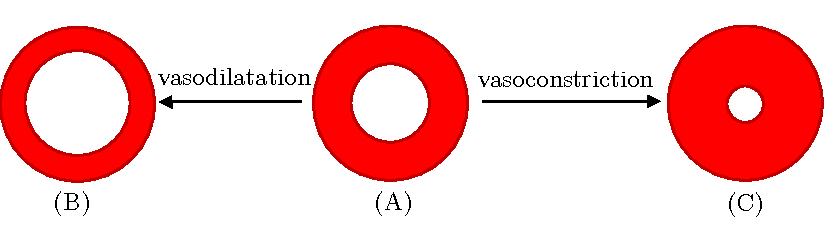
\includegraphics{fig4-14}
    \caption{Schematic representation of the dilatation/constriction process of blood vessels. (A) Cross section of blood vessel in normal state. (B) Vasodilatation process, the size of the blood vessel increases, reducing the overall blood pressure (less tension). (C) Vasoconstriction process, the diameter of the blood vessel diminishes, increasing the overall blood pressure. Preventing or treating hypertension can be achieved by either promoting the state (B) (Pro-vasodilatation agents) or by preventing state (C) (Anti-vasoconstriction agents).}
    \label{fig4-14}
\end{figure}

The semantically equivalent ATC category is \emph{Antihypertensives} (C02) and contains single molecules and drug combinations. The drug repositioning hypotheses for this ATC class are listed and interpreted in Table \ref{tab:tablel02} (\url{https://www.ebi.ac.uk/chembl/research/ftc-hypotheses/code/C02}).

\begin{table}[htbp]
\scriptsize
\begin{tabular}{|p{2cm}|p{2cm}|p{2cm}|p{3cm}|p{4cm}|}
\hline
\textbf{Identifier reference drug} & \textbf{ATC code reference drug} & \textbf{Identifier hypothesis} & \textbf{ATC code hypothesis} & \textbf{Hypothesis interpretation} \\ \hline
DB00457 (Prazosin) & C02 (Antihypertensives) & DB01162 (terazosin) & G04 (Urologicals) & Valid hypotheses, the drug is used as such already \\ \hline
DB00590 (doxazosin) & " & " & " & " \\ \hline
Centrally active hypotensive agents (group A) & " & DB00668 (Epinephrine) & A01 (Stomatological preparations) 
B02 (Antihemorrhagics)
C01 (Cardiac therapy)
R01 (Nasal preparations)
R03 (Drugs for obstructive airway diseases)
S01 (Ophthalmologic) & Drug involved in numerous process, effect varies with quantities, to verify pro-drugs and how it influences \\ \hline
" & " & DB00368 (Norepinephrine) & C01 (Cardiac therapy) & Related therapeutic group, central hormone \\ \hline
" & " & DB00697 (tizanidine) & M03 (Muscle relaxants) & Management of spasticity, same receptors but different locations, inhibition of motoreurons \\ \hline
" & " & DB00320 (Dihydroergotamine) & N02 (Analgesics) & Migraine therapy, vasoconstrictor \\ \hline
" & " & DB00413 (Pramipexole) & N04 (Anti-parkinson drugs) & For Parkinson's disease and restless syndrome. Used off-label for cluster headache. Effect on vaconstriction? \\ \hline
" & " & DB00633 (Dexmedetomidine) & N05 (Psycholeptics) & Because of its pain killing action, it also decreases the blood pressure and heart rate, different location of receptor triggers different effect \\ \hline
" & " & DB01577 (Methamphetamine) & N06 (Psychoanaleptics) & Plausible, illegal molecule \\ \hline
" & " & DB04948 (Lofexidine) & N07 (Other nervous system drugs) & Adrenergic agonist, reported as short-acting antihypertensive, but mostly used to relieve opiate dependency, usage already reported \\ \hline
" & " & DB00935 (Oxymetazoline) & R01 (Nasal preparations)
S01 (Opthalmologicals) & Vasoconstrictor to relieve nasal congestion. Also used for ocular inflammation. \\ \hline
" & " & DB06711 (Naphazoline) & " & " \\ \hline
" & " & DB06694 (Xylometazoline) & " & Nasal vasoconstrictor decongestant \\ \hline
" & " & DB00397 (Phenylpropanolamine) & R01 (Nasal preparations) & Produces vasoconstriction \\ \hline
" & " & DB00964 (Apraclonidine) & S01 (Opthalmologicals) & Used in glaucoma therapy, anti-hypertensive drug in the eye system\\ \hline
" & " & DB00484 (Brimonidine) & " & " \\ \hline
" & " & DB00449 (Dipivefrin) & " & " \\ \hline
\end{tabular}
\caption{Drug repositioning hypotheses related to hypertension (ATC code C02). The symbol " refers to the value of the previous cell.}
\label{tab:tablel02}
\end{table}

The presence of neurological drugs is explainable by their adrenergic side activity; such molecules bind receptors that are similar to the ones involved in blood pressure regulation, yet are located in different parts of the body and produce a different therapeutic effect. A similar pattern is observed with ophthalmological agents, administered for glaucoma, a disease closely related to eye hypertension \citep{quigley1996number}. In this case too, vasodilators are prescribed, but the delivery and formulation of the molecule confers the specificity of the effect. This evidence supports the validity of the hypotheses; administering the drugs in the cardiovascular system rather than in the eye would probably reduce the overall blood pressure.

A series of arguably good hypotheses are related to compounds used against nasal congestion. Their reported pharmacological effect, vasoconstriction of the nose's arteries \citep{bende1996effect}, is the opposite of the one wanted. However, the biological activity of such compounds is strongly related to that of epinephrine, which is particularly sensitive to concentration \citep{evans2001epinephrine}. Depending on the dosage and the body part concerned, the epinephrine molecule can produce radically different outcomes, from vasoconstriction to vasodilatation. On this basis, the repositioning hypotheses related to nasal preparations seem more plausible; still, the delivery methods would need to be adequately optimised.

The information in the FTC helps to group drugs by MoAs as expected, without consideration for the anatomical part acted upon. In order to be repurposed, the delivery mechanisms of the drugs need to be adapted to transport the molecule to the right place in the body. The FTC provides abstract level MoAs, such as the ones presented in this section. It is also possible to use the resource to investigate more detailed mechanisms, as discussed in the coming parts.

\begin{figure}[H]
    \centering
    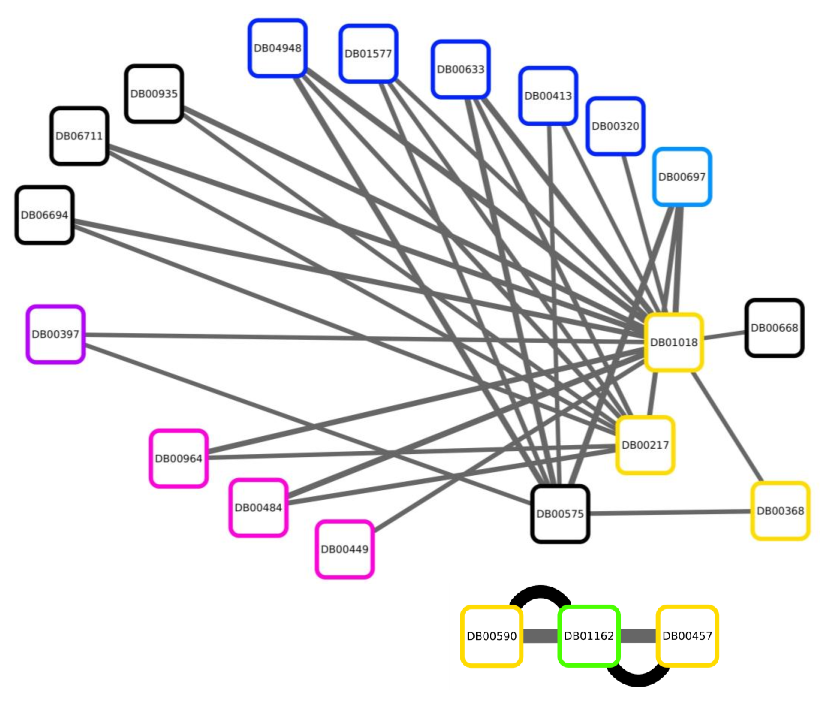
\includegraphics{fig4-15}
    \caption{Drug repositioning hypotheses related to the ATC category C02 - \emph{Anti-hypertensives}. The width of grey edges is proportional to the functional similarity values between drugs. Legend for colours and drug name are available online and in Table \ref{tab:tablel02}.}
    \label{fig4-15}
\end{figure}

\subsubsection{Calcium channel blockers}
One discovered way to reduce blood pressure is by blocking the entry of ions (calcium mostly but also potassium and chloride) into cardiac muscle cells \citep{swedberg2005task}. Deprived from the ions, the cardiac rhythm decreases and the arteries dilate, leading to a drop in blood tension (Figure \ref{fig4-16}).

\begin{figure}[H]
    \centering
    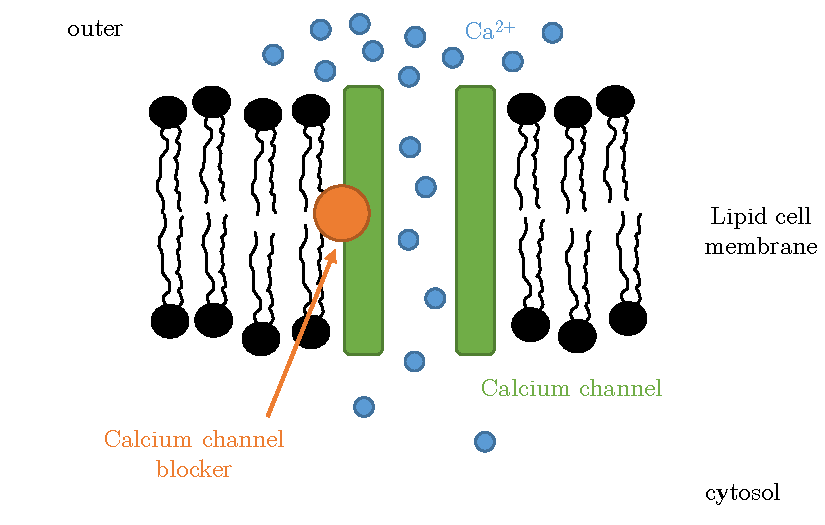
\includegraphics{fig4-16}
    \caption{Schematic illustration of the mechanism of action of calcium channel blockers. The calcium ion is necessary for the contraction of the heart muscle; its releases from internal cellular store or entry inside the cell triggers the contraction. By blocking the channel, the calcium does not circulate any more and the cardiac rhythm decreases, therefore reducing the blood pressure and improving a hypertension.}
    \label{fig4-16}
\end{figure}

One FTC mechanism is directly related to this action: \emph{Anti-high voltage-gated calcium channel activity agent} (FTC\_A0008331 - 13 drugs). As expected, most of the drugs present in this category are indicated as antihypertensive agents (12 out of 13). The direct superclass of this category is the more generic concept \emph{Anti-voltage-gated calcium channel activity agent} (FTC\_A0005245 - 36 drugs). Interestingly, inside this broader class, a quarter of the drugs (8/36) are anticonvulsants (anti-epilepsy) and further classified as \emph{Anti-low voltage-gated calcium channel activity agent} (FTC\_A0008332). This observation reflects the therapeutic closeness between this series of compounds; the two channel types (low and high voltage) can produce radically different physiological outcome from similar structures. The drug flunarizine is a good illustration of this overlapping pharmacology, as it can indeed be indicated as vasodilator or anticonvulsant (\url{https://www.ebi.ac.uk/chembl/ftc/agent/DB04841}), because it interacts non-specifically with either of these channels and can trigger the two response types \citep{van1978effect}.

The corresponding ATC category is C08, the \emph{Calcium channel blockers}. Some repositioning hypotheses have been extracted for this category and are displayed in Table \ref{tab:tablec08}. 

\begin{table}[htbp]
\scriptsize
\begin{tabular}{|p{2cm}|p{2cm}|p{2cm}|p{3cm}|p{4cm}|}
\hline
\textbf{Identifier reference drug} & \textbf{ATC code reference drug} & \textbf{Identifier hypothesis drug} & \textbf{ATC code hypothesis drug} & \textbf{Hypothesis interpretation} \\ \hline
DB00393 (Nimodipine) & C08 (Calcium channel blockers) & DB00379 (Mexiletine) & C01 (Cardiac therapy) & Similar therapeutic categories (potential effect) \\ \hline
DB00661 (Verapamil) & " & DB00308 (Ibutilide) & C01 (Cardiac therapy) & Similar therapeutic categories (potential effect) \\ \hline
DB01115 (Nifedipine) & " & DB01429 (Aprindine) & C01 (Cardiac therapy) & Similar therapeutic categories (potential effect) \\ \hline
" & " & DB00527 (Dibucaine) & S01 (Ophthalmologicals)
D04 (Antipruritics)
C05 (Vasoprotectives)
S02 (Otologicals)
N01 (Anesthetics) & Same MoA, different anatomical location \\ \hline
\end{tabular}
\caption{Drug repositioning hypotheses related calcium channel blockers (ATC code C08). The symbol " refers to the value of the previous cell.}
\label{tab:tablec08}
\end{table}

Mexiletine, ibutilide and aprindine are all used in generic cardiac therapy and arrhythmia; it is therefore not so surprising to find these drugs as hypothesised calcium channel blockers. More interestingly, dibucaine is present in the list. This drug is traditionally used as an anaesthetic and inhibitor of the sodium pump. Because of these closely related mechanisms of action, the compound is also sometimes used as a vasoprotective, to prevent haemorrhoids for instance. This alternative pharmacology provides evidence about the potential role of this drug for hypertension, which can be further investigated.

\begin{figure}[H]
    \centering
    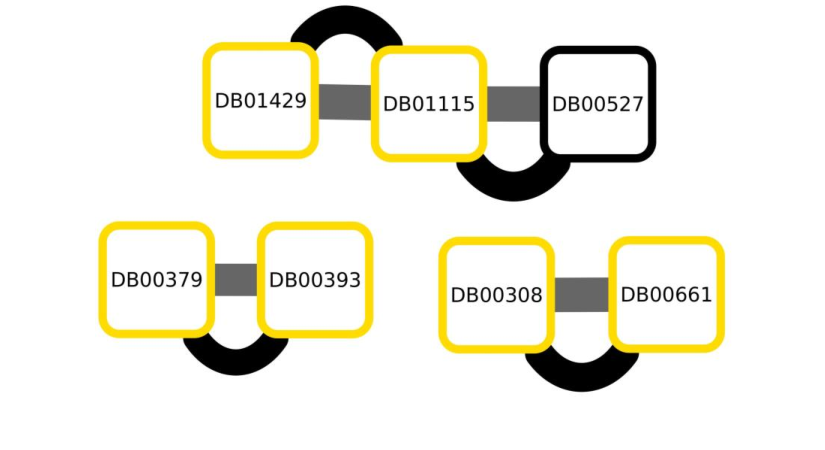
\includegraphics{fig4-17}
    \caption{Drug repositioning hypotheses related to the ATC category C08 - \emph{Calcium channel blockers}. The width of grey edges is proportional to the functional similarity values between drugs. The black lines represent the structural similarities. Legend for colours and drug name are available online and on the Table \ref{tab:tablec08}.}
    \label{fig4-17}
\end{figure}

\subsubsection{Adrenergic receptor antagonists}
Lowering blood pressure can also be achieved by preventing the signal transmission mediated by adrenergic receptors, although such agents are principally used to regulate cardiac dysrhythmia.
There are different subtypes of adrenergic receptor antagonists, listed as subclasses of the FTC category \emph{Anti-adrenergic receptor activity agent} (FTC\_A0004935). The FTC provides a granular representation of this system, first by making the distinction between alpha and beta receptors, and additionally by differentiating the subtype numbers (alpha1 and 2, beta1, 2 and 3).

The corresponding ATC class for this MoA is C07 or \emph{Beta blocking agents} and does not offer such a detailed view on the pharmacological action. Repurposing hypotheses are shown in Table \ref{tab:tablec07} and Figure \ref{fig4-18}.

\begin{table}[htbp]
\scriptsize
\begin{tabular}{|p{2cm}|p{2cm}|p{2cm}|p{3cm}|p{4cm}|}
\hline
\textbf{Identifier reference drug} & \textbf{ATC code reference drug} & \textbf{Identifier hypothesis drug} & \textbf{ATC code hypothesis drug} & \textbf{Hypothesis interpretation} \\ \hline
Beta1 adrenergic antagonists (group A) & C07 (Beta blocking agent) & DB01210 (Levobunolol) & S01 (Ophthalmologicals) & Same MoA, different anatomical location \\ \hline
" & " & DB01214 (Metipranolol) & " & " \\ \hline
DB00489 (Sotalol) & " & DB01118 (Amiodarone) & C01 (Cardiac therapy) & Similar therapeutic categories (known effect) \\ \hline
Beta1 adrenergic antagonists (group C) & " & Bronchodilators (group B) & R03 (Drugs for obstructive airway diseases) & Same MoA, different anatomical location \\ \hline
" & " & DB00841 (Dobutamine) & C01 (Cardiac therapy) & Similar therapeutic categories (known effect) \\ \hline
" & " & DB01102 (Arbutamine) & " & Similar therapeutic categories (known effect) \\ \hline
" & " & DB01288 (Fenoterol) & G02 (Other gynaecologicals)
R03 (Drugs for obstructive airway diseases) & Same MoA, different anatomical location \\ \hline
\end{tabular}
\caption{Drug repositioning hypotheses related \emph{Beat-blocking agents} (ATC code C07). The symbol " refers to the value of the previous cell.}
\label{tab:tablec07}
\end{table}

Some of the listed compounds have an already-reported antihypertensive effect, such as amiodarone, dobutamine and arbutamine, and are more generally used in cardiac therapies. Some other molecules are bronchodilators (group B on Table \ref{tab:tablec07}); they act on the adrenergic receptors expressed in a different location, yet depending on their delivery mechanism they could be potentially active as antihypertensive agents. A couple of drugs (metipranolol and levobunolol) are ophthalmological compounds for the treatment of glaucoma (increased pressure in the eye). These compounds are valid hypotheses for the treatment of hypertension. Here again, the common theme behind the repositioning opportunities is the differences in anatomical locations. The same MoA elicited in a different part of the body can totally change the effect of the drug.

\begin{figure}[H]
    \centering
    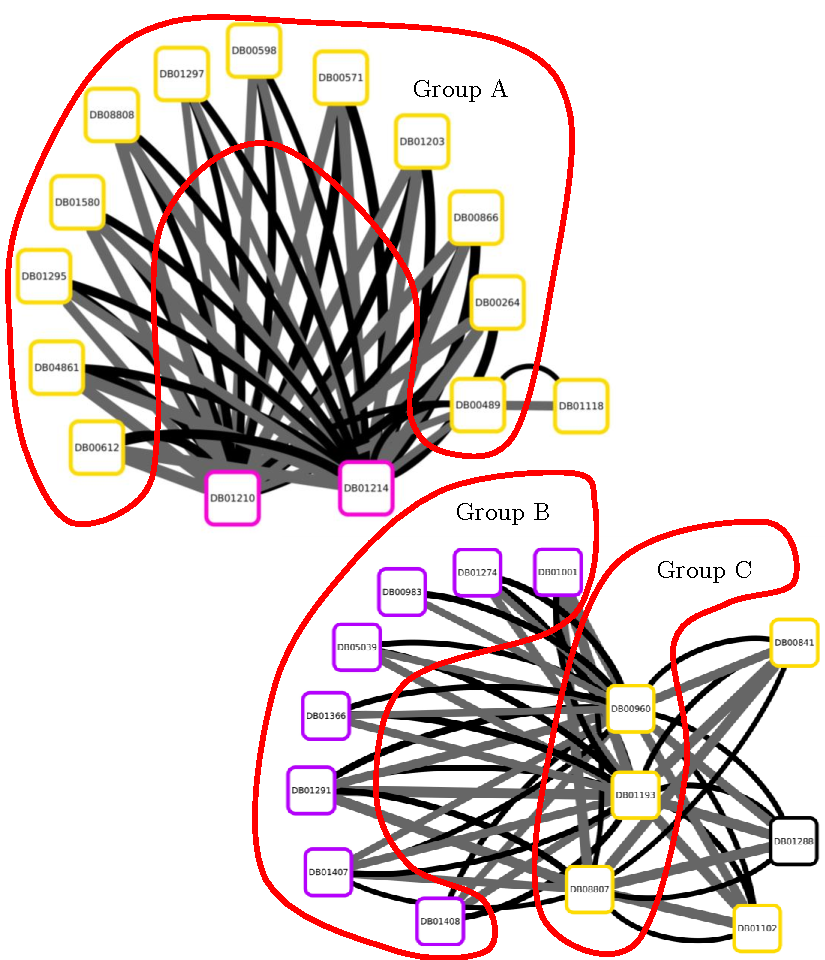
\includegraphics{fig4-18}
    \caption{Drug repositioning hypotheses related to the ATC category C07 - \emph{Beta blocking agents}. The width of grey edges is proportional to the functional similarity values between drugs. The black lines represent the structural similarities. Legend for colours and drug name are available online and on the Table \ref{tab:tablec07}.}
    \label{fig4-18}
\end{figure}

\subsubsection{Alpha-2 agonists}
Acting on alpha2 receptors can lower blood pressure. A stimulation of these receptors, located in the brain, opens the peripheral arteries, which results in better blood circulation throughout the body \citep{swedberg2005task}. The FTC category describing this action is \emph{Pro-alpha2-adrenergic receptor activity agent} (FTC\_P0004938). The 31 drugs classified as such in the FTC have a variety of clinical applications, from sedatives and analgesics to the expected antihypertensive agents (only 6).
No ATC category is dedicated to this mechanism of action, which shows the limit of the gold standard. Even if alpha2 agonists are not the preferred and most common way to reduce hypertension \citep{nelson2010drug}, it is still relevant for drug repositioning purposes to have access to the list of drugs that could act on the receptors, as shown in Table \ref{table:tablealpha}.

\begin{table}[htbp]
\small
\begin{tabular}{|p{5cm}|p{5cm}|}
\hline
\textbf{Action} & \textbf{Number of drugs} \\ \hline
Antihypertensive  & 6 \\ \hline
Dopamine agonist & 9 \\ \hline
Nasal Decongestants (vasoconstrictor) & 6 \\ \hline
Ophthalmologicals & 2 \\ \hline
Analgesics & 3 \\ \hline
Bronchodilator Agents & 2 \\ \hline
Other & 3 \\ \hline
\end{tabular}
\caption{Actions and number of drugs classified as \emph{Pro-alpha2-adrenergic receptor activity agent} (FTC\_P0004938).}
\label{table:tablealpha}
\end{table}

Note that the therapeutic groups to be repurposed belong to several categories that have been previously discussed, such as ophthalmological preparations and bronchodilators, but also to new categories such as dopaminergics, which are notably involved in Alzheimer's disease treatment.

\subsubsection{Diuretics}
Diuretic agents promote the production of urine and help the kidneys to eliminate excess salt and water from the blood. This class of compounds also exhibits vasodilating properties; the exact mechanism of the action is still unclear and not directly related to the salt effect.

The FTC describes at least two mechanisms of action responsible for a diuretic effect: \emph{Anti-sodium:potassium:chloride symporter activity agent} (FTC\_A0008511 - 9 drugs) and \emph{Anti-sodium:chloride symporter activity agent} (FTC\_A0015378 - 7 drugs). All the drugs classified within these categories are all known to be antihypertensive or diuretic agents, without exceptions. The ATC equivalent category is C03 (\emph{diuretics}) which can serve to filter repositioning hypotheses via a similarity analysis. Table \ref{table:tablec03} and Figure \ref{fig4-19} provide a summary of repositioning opportunities related to diuretics.

\begin{table}[htbp]
\scriptsize
\begin{tabular}{|p{2cm}|p{2cm}|p{2cm}|p{3cm}|p{4cm}|}
\hline
\textbf{Identifier reference drug} & \textbf{ATC code reference drug} & \textbf{Identifier hypothesis drug} & \textbf{ATC code hypothesis drug} & \textbf{Hypothesis interpretation} \\ \hline
DB00421 (Spironolactone) & C04 (Diuretics) & DB00665 (Nilutamide) & L02 (Antineoplastics) & Shared off-target \\ \hline
" & " & DB00499 (Flutamide) & L02 (Antineoplastics) & " \\ \hline
" & " & DB01128 (Bicalutamide) & L02 (Antineoplastics) & " \\ \hline
" & " & DB04839 (Cyproterone) & G03 (Sex hormones and modulators of the genital system) & " \\ \hline
\end{tabular}
\caption{Drug repositioning hypotheses related to \emph{Diuretics} (ATC code C03). The symbol " refers to the value of the previous cell.}
\label{table:tablec03}
\end{table}

Three drugs (nilutamide, flutamide and bicalutamide) are currently classified as antineoplastic agents and deemed to be also active as antihypertensive via diuretic effect. These predictions are based on the binding of the drugs to the androgen receptor, which has been shown to be tightly linked to the renin-angiotensin system behind the diuretic activity \citep{ikeda2009androgen} \citep{hoshino2011regulation}. Moreover this receptor is an off-target of spironolactone, the known diuretic drug in the pairs (see Table \ref{table:tablec03}). The last prediction is cyproterone, which is also an androgen receptor antagonist and is currently used for the treatment of hypersexuality and prostatic carcinoma. Its diuretic activity can be explained in the same manner as the other predictions.

\begin{figure}[H]
    \centering
    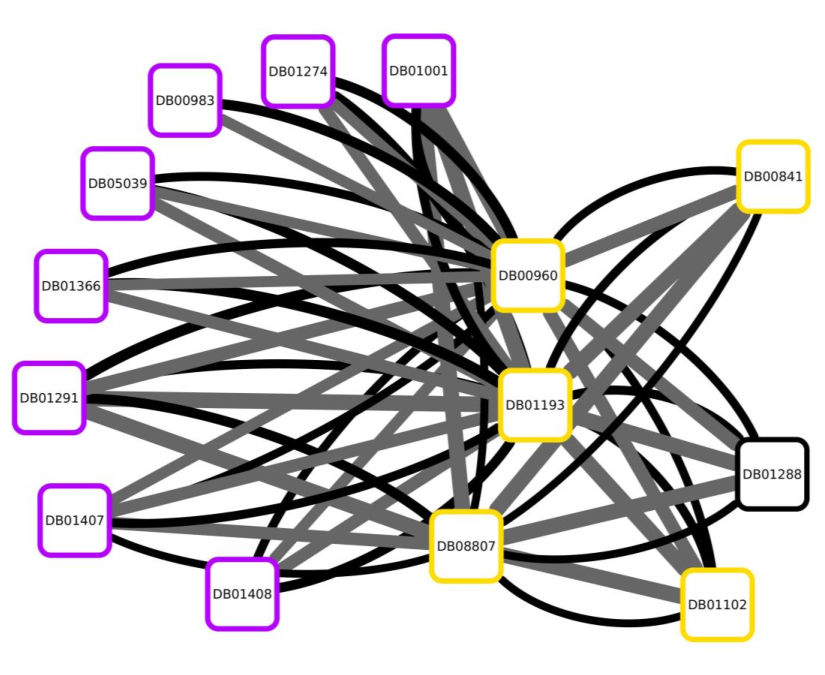
\includegraphics{fig4-19}
    \caption{Drug repositioning hypotheses related to the ATC category C03 - \emph{Diuretics}. The width of grey edges is proportional to the functional similarity values between drugs. The black lines represent the structural similarities. Legend for colours and drug name are available online and on the Table \ref{table:tablec03}.}
    \label{fig4-19}
\end{figure}

\subsubsection{Renin-angiotensin system}
The control of salt and water levels in the blood is accomplished by a pathway known as the renin-angiotensin system (see Figure \ref{fig4-21}).

\begin{figure}[H]
    \centering
    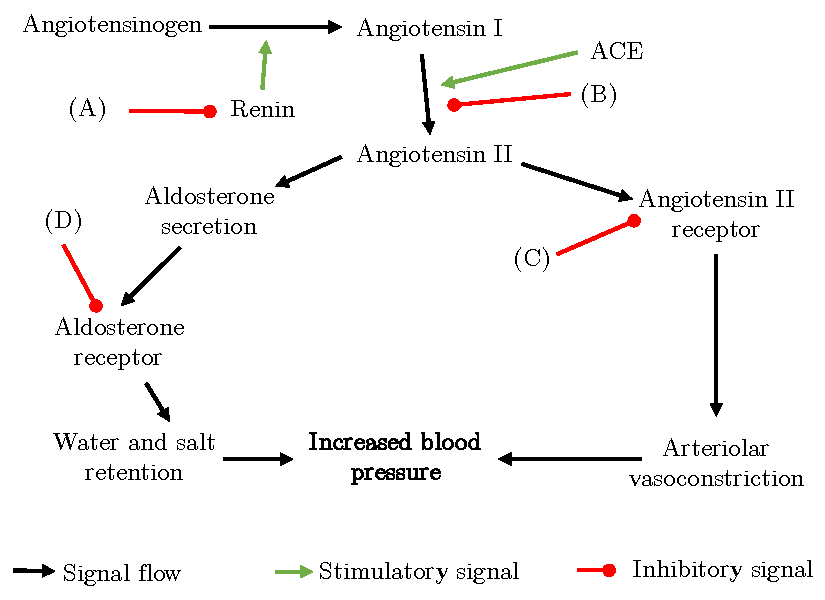
\includegraphics{fig4-21}
    \caption{Simplified summary of the renin-angiotensin system and its implication in blood pressure regulation. Therapeutic intervention points are indicated with a letter. (A) Renin inhibitors: preventing the synthesis of renin reduces the blood pressure. (B) Angiotensin-converting enzyme (ACE) inhibitors: inhibiting the enzymatic activity prevents the synthesis of angiotensin II and decreases the blood pressure. (C) Angiotensin II receptor agonists: blocks the action of the angiotensin II and reduces blood pressure. (D) Aldosterone receptor antagonists: aldosterone signalling promotes water and salt retention and increases the blood pressure. Preventing its action help to release hypertension.}
    \label{fig4-21}
\end{figure}

\paragraph{\textbf{Angiotensin-converting enzyme (ACE) inhibitors}\\}
The angiotensin-converting enzyme (ACE) is the primary target of a series of antihypertensive agents. The enzyme converts angiotensin I into II, a molecule with vasoconstricting properties. Inhibiting the enzymatic activity therefore prevents vasoconstriction and reduces blood pressure (see Figure \ref{fig4-21}-B).
The FTC shows limitations in capturing this specific activity. The closest category is \emph{Anti-peptidyl-dipeptidase activity agent} (FTC\_A0008241 - 14 drugs), describing the generic chemical catalysis performed by the enzyme. Despite being broadly defined, the 14 drugs present in the class are all antihypertensive agents and manually classified as ACE inhibitors in DrugBank. The ATC better defines the mechanism of action, as showed by the class C09AA (\emph{ACE inhibitors, plain}). Because of the specificity of the pharmacology, no drug repositioning hypotheses were analysed for this mechanism of action, yet the action is captured in the FTC and usable for further exploration.

\paragraph{\textbf{Angiotensin II receptor antagonists}\\}
The binding of the angiotensin II molecule to receptors triggers arteriolar vasoconstriction. As shown with ACE inhibition in the previous section, preventing angiotensin II synthesis can promote vasodilatation. Another mechanism to lower blood pressure consists of preventing the binding of angiotensin II to its receptor using an antagonist or \emph{blocker} (see Figure \ref{fig4-21}-C).

The FTC contains a category directly capturing this MoA: \emph{Anti-angiotensin type II receptor activity agent} (FTC\_A0004945 - 11 drugs). Here again all the drugs are indexed as antihypertensive agents and more precisely as angiotensin II receptor antagonists in DrugBank and in the literature. The category does not contain any unexpected results, therefore no repositioning hypotheses can be advanced using this FTC category alone. The ATC contains a detailed representation of the MoA of interest as well, namely the category C09C or \emph{angiotensin II antagonists, plain}.

\paragraph{\textbf{Renin inhibitors}\\}
Renin is a protein present upstream of the vasoconstriction cascade. In order to be physiologically active and elicit vasoconstriction, renin needs first to be synthesised and produced. Inhibiting its production or modification to its active form therefore prevents vasoconstriction signalling and results in decreased blood pressure (see Figure \ref{fig4-21}-A).

One FTC class only provides information about renin: \emph{Anti-renin secretion into blood stream agent} (FTC\_A0002001). This class does not capture the exact MoA by which vasoconstriction is prevented, and no approved drugs have been classified inside this category. This result highlights a limit of the FTC, i.e. more obscure and less common MoAs are not necessarily described in the resource. On the contrary, the ATC features a class for this concept: C09XA, the \emph{renin-inhibitors}.

\paragraph{\textbf{Aldosterone receptor antagonists}\\}
Aldosterone is a hormone secreted by the adrenal gland, located in the cortex. The molecule is involved in signalling which positively regulates blood pressure. Preventing its activity decreases blood pressure; consequently aldosterone receptor antagonists can improve hypertension (see Figure \ref{fig4-21}-D).

This MoA is less traditional than the ones introduced previously in the treatment of hypertension; nonetheless there exist some approved drugs relying on it and described in the ATC: C03DA \emph{Aldosterone antagonists} (4 drugs). Unfortunately such a resolution is not available in the FTC. Two categories merely describe bioprocesses in which aldosterone is involved: \emph{Anti-aldosterone metabolic process agent} (FTC\_A0032341) and \emph{Anti-aldosterone secretion agent} (FTC\_A0035932), which do not capture the exact MoA nor contain any drugs. This MoA shows again a limitation of the FTC for less frequently used therapeutic categories, as in the previous section.

\subsubsection{Peripheral vasodilators}
Vasodilators are most commonly prescribed for heart problems, but they are also used to treat conditions affecting the blood vessels located in peripheral parts of the body, such as the arms and legs. Raynaud's disease is an example of a condition where peripheral arteries face difficulties to maintain the blood supply, resulting in a numb feeling in the patient when exposed to stress or cold temperatures.

The FTC does not contain a category directly related to this type of action. Indeed, the anatomical location of the pharmacological effect is not covered in the classification; it is therefore impossible to distinguish a peripheral vasodilation from a generic vasodilatation event. On the contrary, the ATC contains a category describing the \emph{peripheral vasodilators} (C04), which can serve to investigate drug repositioning hypotheses (\url{https://www.ebi.ac.uk/chembl/research/ftc-hypotheses/code/C04}). The generated hypotheses are listed in Table \ref{table:tablec04} and shown in Figure \ref{fig4-22}.

\begin{table}[htbp]
\scriptsize
\begin{tabular}{|p{2cm}|p{2cm}|p{2cm}|p{3cm}|p{4cm}|}
\hline
\textbf{Identifier reference drug} & \textbf{ATC code reference drug} & \textbf{Identifier hypothesis drug} & \textbf{ATC code hypothesis drug} & \textbf{Hypothesis interpretation} \\ \hline
Drugs used as peripheral vasodilators, group A & C04 (Peripheral vasodilators) & DB06148 (Mianserin) & N06 Psychoanaleptics (Arousing effect) & Known to produce a range of vascular effect according to drugbank \\ \hline
" & " & DB00656 (Trazodone) & " & " \\ \hline
" & " & DB00370 (Mirtazapine) & " & " \\ \hline
" & " & DB01149 (Nefazodone) & " & " \\ \hline
" & " & DB01624 (Zuclopenthixol) & N05 Psycholeptics (Calming effect) & Adrenergic blockade reported from DrugBank, so possible effect on cardiovascular system \\ \hline
" & " & DB01608 (Propericiazine) & " & " \\ \hline
" & " & DB00800 (Fenoldopam) & C01 Cardiac therapy & Same group, known similar action \\ \hline
\end{tabular}
\caption{Drug repositioning hypotheses related to \emph{peripheral vasodilators} (ATC code C04). The symbol " refers to the value of the previous cell.}
\label{table:tablec04}
\end{table}

It appears that most of the repositioning hypotheses derived for this group involve molecules used for neurological disorders. First, the series of psychoanaleptics (arousing agent) is already known to produce a range of vascular effects, giving confidence in the validity of the predictions \citep{khalifa2003zuclopenthixol}. A couple of compounds are psycholeptics (calming agents). The mechanism of action of these drugs relates to adrenergic blockade \citep{khalifa2003zuclopenthixol}; knowing the involvement of the adrenergic receptors in vasoconstriction (cf previous sections), these two psycholeptic agents can plausibly have an effect on peripheral arteries. The last prediction concerns fenoldopam, a drug used in cardiac therapy. The original indication is functionally close to the new predicted one; an activity in the peripheral blood stream is therefore likely to be observed.

\begin{figure}[H]
    \centering
    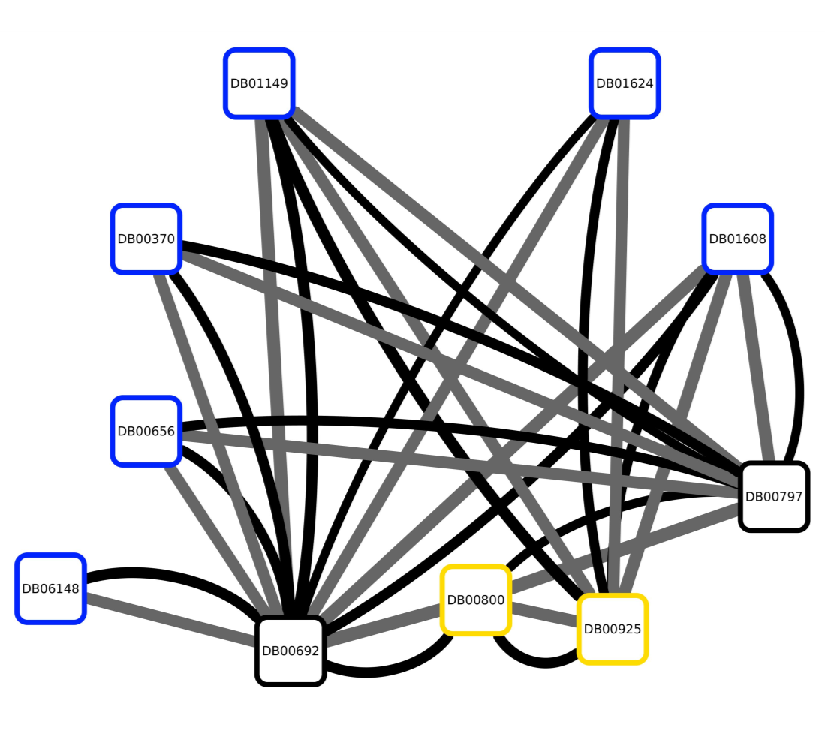
\includegraphics{fig4-22}
    \caption{Drug repositioning hypotheses related to the ATC category C04 - \emph{Peripheral vasodilators}. The width of grey edges is proportional to the functional similarity values between drugs. The black lines represent the structural similarities. Legend for colours and drug name are available online and on the Table \ref{table:tablec04}.}
    \label{fig4-22}
\end{figure}

The repositioning hypotheses generated for this group highlight the close relation between neurologicals and vasodilators. Two of the compounds clinically used as peripheral vasodilators (phentolamine and tolazoline) are also already used to treat muscular and joint pains. From this observation, it appears legitimate for other neurological agents to be active in cardiovascular vasodilation.

As a side note for future work, predictions involving neurological drugs are difficult to validate experimentally. The commercial distribution of such molecules is indeed rigidly regulated in most countries, as this class of compounds can also be consumed for illicit recreational use.

The treatment of cardiac hypertension can be addressed from various conceptual angles, as presented in this section. For some cases, the FTC describes these abstract MoAs; in such scenarios, the drugs classified in the corresponding FTC category are candidates capable of triggering the given pharmacological effect. This methodology is the toolbox approach, and was not directly used here to derive drug repositioning hypotheses, yet it will be presented in a later section on Alzheimer's disease. On the other hand, some of the conceptually sought MoAs are present in the categories of the gold standard ATC. In such cases repositioning hypotheses can be investigated using the similarity-based approach, as shown in this section using the hypotheses previously generated and available through the web application (see section \ref{sec:opendrug}).

The drug repositioning hypotheses predicted for cardiovascular hypertension are rooted in similar bioactivity but different anatomical location. For instance, drugs currently indicated for glaucoma, pulmonary problems or against nasal congestion were all listed in the repositioning predictions. These molecules all potentially exhibit vasoconstrictive properties and can further be investigated for the predicted new indication.

\subsection{Repositioning for Alzheimer's disease}
The content of the FTC and the open repositioning hypotheses derived from it can be applied to a wide variety of human diseases. Previous sections exemplified an analysis on vascular hypertension and on the repurposing hypotheses derived using similarity-based methods. In this section, I wanted to show to the reader how the toolbox approach can also provide valuable hypotheses for a dementia currently with no cure: Alzheimer's disease. The technique presented here makes use of the FTC categories as analogues to compartments of a toolbox, helping to find drugs to address the condition, as motivated in Chapter 2.

Alzheimer's disease is a neurodegenerative dementia with a relatively poorly understood biology \citep{mckhann2011diagnosis}. Phenotypic manifestations include progressive appearance of plaques and tangles in the brain. On the molecular level, several hypotheses are currently under investigation \citep{mckhann2011diagnosis}. Briefly, two macromolecules appear to be strongly involved in the disease: beta-amyloid peptides, the main component of some of the deposits found in patients' brains, and the Tau protein, responsible for stabilising microtubules \citep{scheuner1996secreted} \citep{delacourte1986alzheimer}. Given this summary knowledge on the topic, the goal of the following analysis is to extract from the FTC the MoAs directly related to these two proteins, in order to subsequently identify approved drugs capable of perturbing the dementia.

Five FTC categories containing drugs are directly related to the biological processes of the neurodegenerative condition: \emph{Anti-amyloid precursor protein-biosynthetic-process agent} (FTC\_A0042983), \emph{Anti-Tau protein kinase-activity agent} (FTC\_A0050321), \emph{Anti-Tau protein binding agent} (FTC\_A0048156), \emph{Anti-beta amyloid binding agent} (FTC\_A0001540) and finally \emph{Pro-beta amyloid binding agent} (FTC\_P0001540). I considered the drugs present inside each of these classes as potential candidates to be repurposed. Table \ref{table:alz} shows these drugs, which have been further manually grouped based on the overall similarity of their actions (numbers in Table \ref{table:alz}).


\begin{table}[htbp]
\scriptsize
\begin{tabular}{|p{2.5cm}|p{2.5cm}|p{2.5cm}|p{2.5cm}|p{2.5cm}|}
\hline
\textbf{(A) Anti-beta-amyloid binding agent} & \textbf{(B) Pro-beta-amyloid binding agent} & \textbf{(C) Anti-tau protein binding agent} & \textbf{(D) Anti-tau protein kinase activity agent} & \textbf{(E) Anti-amyloid precursor protein biosynthetic process agent} \\ \hline
\textbf{Subgroup 1} & Pralidoxime & Vorinostat & Lithium & Hesperetin \\
Malathion & Dipivefrin &  &  & Ezetimibe \\
Echothiopathe & \textbf{Subgroup 5} &  &  &  \\
Hexafluronium & Varenicline &  &  &  \\
\textbf{Subgroup 2} & Nicotine &  &  &  \\ 
Gallamine &  &  &  &  \\ 
Triethiodide &  &  &  &  \\ 
Tubocurarine &  &  &  &  \\ 
\textbf{Subgroup 3} &  &  &  &  \\ 
Isoflurophate &  &  &  &  \\ 
Tacrine &  &  &  &  \\ 
Edrophonium &  &  &  &  \\ 
Galantamine &  &  &  &  \\ 
Ambenonium &  &  &  &  \\ 
Demecarium &  &  &  &  \\ 
Pyridostigmine &  &  &  &  \\ 
Rivastigmine &  &  &  &  \\ 
Donepezil &  &  &  &  \\ 
Physostigmine &  &  &  &  \\ 
Neostigmine &  &  &  &  \\ 
\textbf{Subgroup 4} &  &  &  &  \\ 
Amobarbital &  &  &  &  \\ 
Pentobarbital &  &  &  &  \\ 
Phenobarbital &  &  &  &  \\ 
Thiopental &  &  &  &  \\ 
Talbutal &  &  &  &  \\ 
Butabarbital &  &  &  &  \\ 
Primidone &  &  &  &  \\ 
Metharbital &  &  &  &  \\ 
Butethal &  &  &  &  \\ 
Heptabarbital &  &  &  &  \\ 
Aprobarbital &  &  &  &  \\ 
Hexobarbital &  &  &  &  \\ 
Secobarbital &  &  &  &  \\ 
Butalbital &  &  &  &  \\ 
Metharbital &  &  &  &  \\ 
Mehylphenobarbital &  &  &  &  \\ \hline
\end{tabular}
\caption{FTC categories describing some of the modes of 
action that could impact Alzheimer's disease (letters on figure). The categories have been manually picked on the basis that they could directly affect
the dementia. Drugs classified in these FTC categories further 
manually grouped based on their MoAs similarities (numbers on Figure).}
\label{table:alz}
\end{table}

Within group A, subgroups 1, 2 and 3 are inhibitors of the cholinergic system and some of them, such as galantamine (DB00674), have  already been investigated to treat Alzheimer's disease and other related dementias. This class of agent is in line with the cholinergic hypothesis \citep{babic1999cholinergic}, stating that Alzheimer's disease could be caused by dysfunctions in the processing of the acetylcholine.

Subgroup 4 is exclusively composed of barbiturates (central nervous system depressants). The presence of this pharmacological class of compounds as an Alzheimer's disease treatment is more surprising, as very little literature reports on it. Further investigations reveal that the neuronal acetylcholine receptor subunit alpha-7, a common off-target of barbiturates, binds beta-amyloids with high affinity \citep{wang2000amyloid}. As beta-amyloids are themselves strongly involved in the pathology, barbiturates could affect the state of the condition, similarly to cholinergic inhibitors \citep{wang2000amyloid}.

Group B contains four compounds; nicotine and varenicline have been further grouped together because of similar pharmacology (subgroup 5). Nicotine has been shown to improve some of the symptoms of Alzheimer's disease \citep{jones1992effects}; it is therefore expected to find this molecule in the predictions. Varenicline possesses a pharmacology related to that of nicotine, which would explain the presence of the drug in this category.

The two remaining drugs of group B are pralidoxime and dipivefrin. Little information is available regarding their potential action against the condition, yet these compounds seem linked to the cholinergic hypothesis and could be considered for experimental testing.

Groups C and D contain one molecule each. These compounds have been classified as agents perturbing some of the physiological function of the Tau protein, a key actor in Alzheimer's disease \citep{grundke1986abnormal}. Vorinostat (group C) is currently indicated for the treatment of cutaneous manifestations in patients with T-cell lymphoma, yet a study has shown \emph{in vivo} (mouse model) the potential of the drug and other histone deacetylase inhibitors in regards to memory deficit \citep{kilgore2010inhibitors}. The presence of lithium (group D) was confirmed by a recent study demonstrating a long-term protective effect for the ion in regards to Alzheimer's disease \citep{young2011more}.

The last group, group E, contains ezetimibe and hesperetin. These two compounds are primarily used as cholesterol lowering agents (statins). As cholesterol metabolism in the brain appears to be related to dementia, statins are believed to prevent or improve the symptoms of the patients. Although early studies \citep{wolozin2004cholesterol} have failed to clearly show a beneficial effect, a recent clinical trial of over 58,000 patients revealed the positive effect of high potency statins to prevent dementia \citep{esc13}. Interestingly, this prediction was featured in the FTC before the announcement of the results of the clinical trial.

From the examples briefly presented above, reported and confirmed by the literature, the FTC appears to be suitable to identify real repurposing hypotheses tailored to a disease. Correctly identifying MoAs of interest helps to retrieve the compounds which might impact the treatment of a condition.

\subsection{Comparison of prediction approaches}
In the previous sections, two approaches were discussed: toolbox and similarity-based. The theoretical difference between the methodologies is illustrated in Figure \ref{fig4-13}, yet the actual repositioning hypotheses coming from either methods were not compared. The aim of this section is to discuss the relative advantage of one methodology over the other and discuss the relative distribution of the results.

The toolbox approach main strength resides in the possibility to identify drugs with novel MoA, not necessarily used in clinics yet. For instance, the categories \emph{Anti-neuron death agent} (FTC\_A0070997), \emph{Anti-circadian rhythm agent} (FTC\_A0007623) or \emph{Anti-blood vessel remodeling agent} (FTC\_A0001974) are novel and interesting MoAs which could be desirable for certain type of diseases. The toolbox approach enables the straightforward identification of such agents. On the other hand, and because of the way the FTC is built, the presence of a single annotation in GOA or DrugBank can change whether a drug is classified in a particular FTC category; accordingly, the toolbox approach is therefore more sensitive to the quality of the curated knowledge.

The similarity-based approach is of interest to find potential candidates for a well defined therapeutic group, as described in the ATC and well-known in clinics. The predictions generated use the set of annotations related to a drug, rather than just a discrete category as with the toolbox approach, therefore the prediction should be less sensitive to missing or incomplete knowledge. The similarity values are however relatively derived by comparing a drug to another, therefore it is impossible to find new MoA as with the toolbox approach.

Section \ref{sec:Antihypertensives} presented the drug repositioning hypotheses related to the cardiac hypertension treatment, derived using the two approaches. In this case, from the toolbox method 50 drugs were considered to be active for this MoA, using two FTC classes (\emph{Pro-vasodilation agent} and \emph{Anti-vasoconstriction agent}). With the similarity-based strategy, 16 drugs were predicted by comparing their function to the one of the drugs classified in the ATC category C02 (\emph{Antihypertensives}). Figure \ref{fig4-22bis} displays the list of predicted drugs and their current therapeutic groups.

\begin{figure}[H]
    \centering
    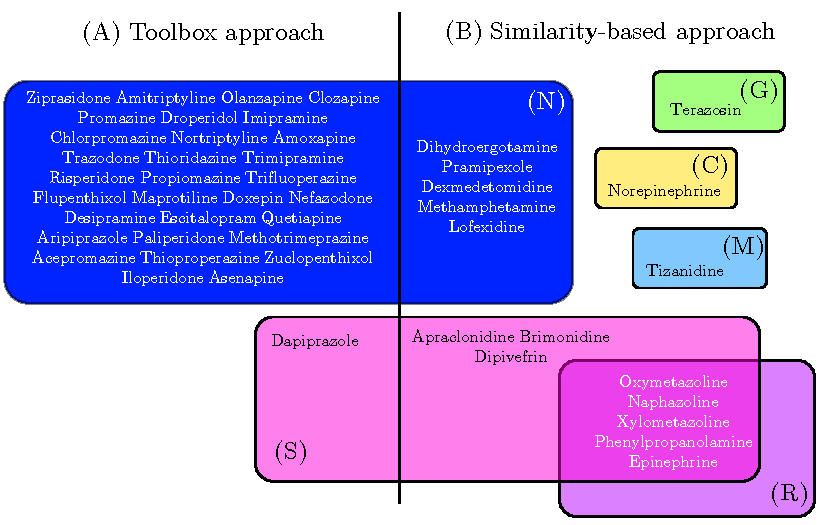
\includegraphics{fig4-22bis}
    \caption{Comparison of the drug repositioning hypotheses generated for the treatment of anti-hypertension, using (A) the toolbox and (B) similarity-based approaches. Letters indicate the ATC therapeutic groups inside which these drugs are currently used. The two methodologies predicted numerous compounds from the \emph{Nervous system} (N).}
    \label{fig4-22bis}
\end{figure}

From the list of 50 drugs generated with the toolbox approach, 18 were drugs already indicated for the treatment of the hypertension. The 32 remaining drug are all compounds indicated for the \emph{Nervous system} an mostly psychoactive drugs. Interestingly, the similarity-based approach predicted drug from this category too, showing an agreement between the methodologies. The similarity-based methodology predicted drugs present in ATC categories not identified by the toolbox approach, with drugs currently indicated for the \emph{Sensory organs} or the \emph{Respiratory system}. There is no overlap regarding the actual predicted drugs, because of the variation of annotations, influencing the predictions as discussed earlier in this section. Both methods predict drugs from similar therapeutic groups to be active (class level), with variation regarding the actual molecule. Taken together these result illustrate the validity of the hypotheses generated and help to better appreciate the features of each methodology introduced.

\section{Summary}
The FTC was developed to address drug repositioning or more generally indication discovery for active molecules. In this chapter, I illustrated the capability of the resource to fulfil its expectations. First, I discussed the relationship between the similarity of the molecular structure, indication and MoA of approved drugs. Within the dataset considered, the functional and structural descriptors chosen can serve as proxies for the similar property principle: on average, drugs prescribed for increasingly specific indications have increasingly similar molecular structures and functions. More importantly, these descriptors can also be used to identify outliers to the rule, in other words, drugs that are functionally similar yet clinically used for different indications. This set of drug pairs was defined as the drug repositioning opportunities. The list is openly available online via a web application and serves to investigate the relationship between therapeutic areas (cf section \ref{sec:isolation}).

The hypotheses cover a wide spectrum of clinical areas, enabling systematic analyses to be performed. However, it is clear that some biological interpretation is still needed on the top of the predictions, in order to understand the molecular reasons behind the MoAs and to move towards laboratory experiments. I therefore decided to focus my attention on two disparate biological dysfunctions: hypertension and Alzheimer's dementia.

From the state-of-the-art presented in Chapter 1, I believe that functional genomics and gene expression experiments are the computational methods that currently produce the most promising results for drug repositioning. I envisioned that this success came from the capacity of these techniques to systematically handle the concept of \emph{function}. In this regard, I specified in Chapter 2 one theoretical approach to studying and handling biomedical knowledge for drug discovery, where organisms are compared to a black box machine to be fixed. I suggested description logics (DLs) as a helpful mathematical framework to address such a task, and in particular the scalable \dl{EL\textsuperscript{++}} family. The theory introduced in Chapter 2 found an implementation in chapter 3 with the FTC. This classification defines the mode and mechanism of actions of a panel of approved drugs and is evaluated against the ATC, the traditionally used standard. Finally, an analysis was performed over the data, leading to the large-scale generation of drug repositioning hypotheses presented in this chapter. The work done during my thesis covers only the very beginning of the long hurdled road towards innovative medicine. Knowing that a new drug takes around 12 years and a billion dollars in investment to reach the market (section 1.1), it would have been unrealistic to think that such a goal would have been reached with the time and money allocated for my work. Nonetheless it is possible and important to set the outcomes of the work in the overall drug discovery process, and to discuss the logical next steps which can be undertaken from the results obtained. This will be covered in the final chapter.

\section{Methods}

\subsection{Structural fingerprints calculation}
\label{sec:structural}
The fingerprint of a molecule is a simplified - or hashed - representation of its structure, namely a one-dimensional array of 0's and 1's (bits). The presence of a 1 in the fingerprint sequence in a particular position means that a chemical group of interest is present in the molecule, while a 0 means that the group is absent. 
Four different implementations of fingerprinting were tested. All of them are featured in the Chemistry Development Kit (CDK). I used the version 1.4.19, downloaded from \url{http://sourceforge.net/projects/cdk/}. The various methods have different rationales, as documented online (\url{http://cdk.github.io/cdk/1.4/docs/api/}).

\begin{itemize}
  \item Hybridization fingerprint: default fingerprinting methodology. Does not take into account aromaticity, instead focuses on SP2 molecular hybridisation.
  \item Extended fingerprint: same as previous, provides support for rings features.
  \item MACCS fingerprint: generates 166 bit MACCS keys \citep{fpdalke}. From a series of SMART patterns, the functions output the presence or absence of particular chemical features.
  \item PubChem fingerprint: generates a large fingerprint (881 bits) from a list of curated rules available online \citep{pubchemfp}.
\end{itemize}

\subsection{Structural similarity between drugs}
\label{sec:structuralsimbet}
The relative structural similarity between a pair of drugs was calculated as the Tanimoto similarity value \citep{tanimoto1958elementary} of their fingerprints. Note that Tanimoto similarity is strongly related to the Jaccard index used to calculate semantic similarity. It is defined in section 2.4.3. The similarity value ranges between 0 (totally dissimilar) and 1 (identical) and was calculated using the CDK.

\subsection{Agreement between fingerprinting methodologies}
\label{sec:agreement}
The respective agreement between the various fingerprinting methodologies listed in section \ref{sec:structuraldescriptorselection} was defined as the value of the Pearson product-moment correlation coefficient. This coefficient \emph{is a measure of the linear correlation (dependence) between two variables X and Y, giving a value between +1 and −1 inclusive, where 1 is total positive correlation, 0 is no correlation, and −1 is negative correlation} \citep{hane1993pearson}. In this case, variable X is the structural similarity values between the fingerprints generated with the same method for all drugs (e.g. all pairwise comparisons of fingerprints generated using the MACCS method). The variable Y has the same content, but the values are calculated using a different method. The value of the coefficient is interpreted as: 0 means total disagreement and 1 total agreement between the two methodologies tested.

As four different methods were tested against all the others, each one of them has three coefficient values, representing the different agreement scores (content of a row in Table \ref{sec:introduction}). The average of these three values was defined as the overall agreement of one method against other methodologies. The higher the average coefficient, the more one method agrees with the others overall.

\subsection{Kernel density plots}
The kernel density estimates were created using the \emph{stats} package in R. From the documentation of the package (\url{http://stat.ethz.ch/R-manual/R-patched/library/stats/html/density.html}) the density method \emph{disperses the mass of the empirical distribution function over a regular grid of at least 512 points and then uses the fast Fourier transform to convolve this approximation with a discretized version of the kernel and then uses linear approximation to evaluate the density at the specified points}. The resulting density of similarity can be seen as a value proportional to the chance of drawing from the population a number that is lying in the close proximity of the similarity value. Gaussian smoothing kernel was always used; other parameters were left to default.

\subsection{Web application related to drug repositioning hypotheses}
The source code of the web application is fully open and available at \url{https://github.com/loopasam/repurposing-analyses}. The application is deployed under \url{https://www.ebi.ac.uk/chembl/research/ftc-hypotheses}. The project was built using the Play! framework and the Brain library \citep{croset2013brain}, mentioned before in this document. Users can browse the drug repositioning hypotheses in the application, as illustrated in the screen shot Figure \ref{fig4-23}.

\begin{figure}[ht]
    \centering
    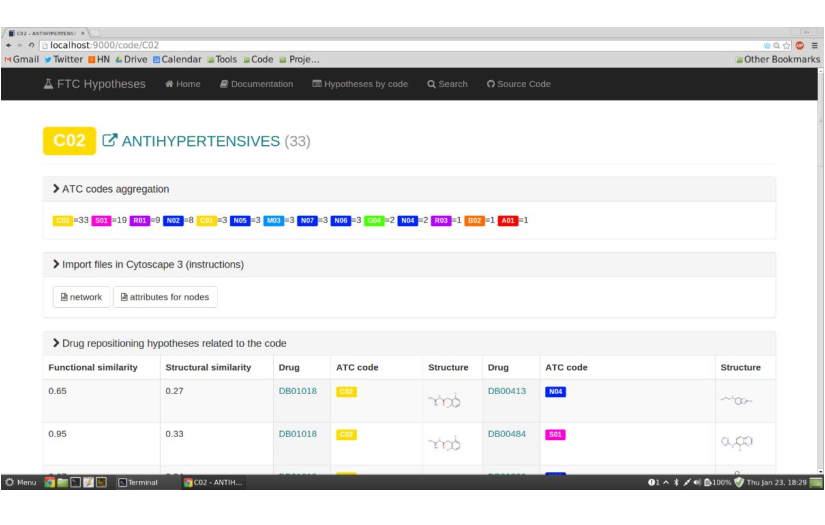
\includegraphics{fig4-23}
    \caption{Screen shot of the web application to explore drug repositioning hypotheses. The hypotheses are accessible online at \url{https://www.ebi.ac.uk/chembl/research/ftc-hypotheses}}
    \label{fig4-23}
\end{figure}

The hypotheses are accessible from either the ATC code they relate to or by the DrugBank code of the drugs involved in the prediction. The user has the possibility to download the network of predictions as a flat file, for further processing by a tool such as Cytoscape for instance.

\subsection{Filtering of drug repositioning hypotheses}
\label{sec:filteringof}
The list of drug pairs associated in different ATC groups with a resolution of two levels is the starting set used to generate the hypotheses (corresponding to the pairs plotted on Figure \ref{fig4-5} panel B). I considered the ATC level 2 as a good characterisation of a drug's indication. From this dataset, only the values with a functional similarity superior to 0.6 were conserved. All the other data points were discarded. In this filtered subset, some of the drugs have very few functional annotations; in such cases it is often not clear whether the high functional similarity is biologically meaningful or artefactual and coming from the semantic similarity methodology. In order to filter these ambiguous cases out, I removed all drugs present directly or indirectly in less than 13 FTC classes. The decision is arbitrary and derived from observations and interpretations made over the data. This heuristic aims at first removing the noise, and second discarding drugs about which little is known from a data-centric perspective.

\subsection{Filtering of relationships between therapeutic areas}
\label{sec:filteringofthe}
The list of drug repositioning hypotheses was used to analyse the links between therapeutic domains. On Figure \ref{fig4-11} (abstracted - one level), the therapeutic areas have been grouped or abstracted according to their direct ATC super classes. For example, a hypothesis containing drugs indicated for the ATC code A01 and M01 was simplified as a link between the category A and M. The more times a link is present between two ATC groups (first level), the more related these two groups are. When this strength of association was below 25, the association was discarded. This choice is arbitrary and was made in order to remove the noise and extract the most salient features of the dataset.

Figure \ref{fig4-12} (two levels trimmed) is built from the same data as Figure \ref{fig4-10}, but by removing all the links with a strength inferior to 15 associations. This threshold is also arbitrary and was applied in order to clarify the overall connectivity pattern and look at the most prominent associations.
